\documentclass[11pt]{amsart}

\usepackage[T1]{fontenc}
\usepackage{lmodern}
\usepackage[a4paper,hmargin=1.15in,vmargin=1.1in]{geometry}
\usepackage{amssymb}
\usepackage{graphicx}
\usepackage{booktabs}
\usepackage{xcolor}
\usepackage{enumitem}
\usepackage{microtype}
\usepackage[colorlinks=true,linkcolor=blue!50!black,citecolor=blue!50!black,urlcolor=blue!50!black,bookmarksnumbered=true]{hyperref}
\usepackage{xurl}
\graphicspath{{./}{../}}

\tolerance=2000
\emergencystretch=2em
\raggedbottom

\newtheorem{theorem}{Theorem}[section]
\newtheorem{lemma}[theorem]{Lemma}
\newtheorem{proposition}[theorem]{Proposition}
\newtheorem{corollary}[theorem]{Corollary}
\theoremstyle{definition}
\newtheorem{definition}[theorem]{Definition}
\theoremstyle{remark}
\newtheorem{remark}[theorem]{Remark}
\numberwithin{equation}{section}

\newcommand{\R}{\mathbb{R}}
\newcommand{\Z}{\mathbb{Z}}
\newcommand{\C}{\mathbb{C}}
\newcommand{\E}{\mathbb{E}}
\newcommand{\SU}{\mathrm{SU}}
\newcommand{\SO}{\mathrm{SO}}
\newcommand{\U}{\mathrm{U}}
\newcommand{\g}{\mathfrak{g}}
\newcommand{\Tr}{\operatorname{Tr}}
\newcommand{\ReTr}{\operatorname{Re}\operatorname{Tr}}
\newcommand{\ImTr}{\operatorname{Im}\operatorname{Tr}}
\newcommand{\Hess}{\operatorname{Hess}}
\newcommand{\Ric}{\operatorname{Ric}}
\newcommand{\Cov}{\operatorname{Cov}}
\newcommand{\Var}{\operatorname{Var}}
\newcommand{\dist}{\operatorname{dist}}
\newcommand{\ip}[2]{\langle #1,#2\rangle}

\begin{document}

\title[Lattice Yang--Mills theory in a forest gauge]{Mass Gap of
Four-Dimensional Lattice Yang--Mills Theory in a Forest Gauge}

\author[D. Bhattacharjee]{Deep Bhattacharjee}
\address{Formerly, Electro-Gravitational Space Propulsion Laboratory
(EGSPL), Bhubaneswar, Odisha 751030, India; formerly, University of
Calcutta, Senate House, 87/1 College Street, Kolkata 700073, West Bengal,
India}
\email{itsdeep@live.com, d.bhattacharjee@erl-forschung.de}
\urladdr{\href{https://orcid.org/0000-0003-0466-750X}{orcid.org/0000-0003-0466-750X}}
\thanks{Corresponding author: Deep Bhattacharjee.}

\author[U. Bhattacharya]{Ushashi Bhattacharya}
\address{Formerly, National Taiwan University, Taipei 106319, Taiwan}
\email{rai.bhattacharya.in@gmail.com}
\urladdr{\href{https://orcid.org/0009-0002-2254-3914}{orcid.org/0009-0002-2254-3914}}

\date{20 October 2026}

\subjclass[2020]{Primary 81T25, 82B20; Secondary 60K35, 81T13, 22E30,
58J50, 65G30}
\keywords{Lattice gauge theory, gauge fixing, Dobrushin uniqueness, mass
gap}

\begin{abstract}
\itshape
We fix the gauge of four-dimensional lattice Yang--Mills theory on a field
of straight lines that meets every plaquette in exactly one link, so that
each free link interacts with twelve others instead of eighteen. In this
gauge the theory has a unique infinite-volume state with exponential decay
of correlations and a positive mass gap at fixed lattice spacing, for SU(2)
beyond the limit of every single-link argument in a gauge of this kind, by
blocks made of the three free links of a plaquette, for
every SU(N) beyond the curvature limit of the ungauged theory, and for SU(3)
on a range more than two and a half times as large as was known before,
where the same blocks raise the gap at the end of that range by two orders
of magnitude and carry the range past it to $\beta_W=0.76$.
\end{abstract}

\maketitle

\setcounter{tocdepth}{1}
\tableofcontents


\section{Introduction}\label{sec:intro}

Wilson's lattice gauge theory~\cite{Wil74} assigns an element $Q_e$ of a
compact group $G\subset\U(N)$ to every link $e$ of $\Z^4$ and weighs a
configuration by $\exp(N\beta\sum_p\ReTr Q_p)$, where $Q_p$ is the ordered
product of the four link variables around the plaquette~$p$.\footnote{This is
the normalisation of Shen, Zhu and Zhu~\cite{SZZ23} and of our earlier
paper~\cite{BB26a}. The conventional inverse coupling is $\beta_W=N^2\beta$,
so the weight is $\exp(\frac{\beta_W}N\sum_p\ReTr Q_p)$; for $\SU(2)$,
identified with the unit quaternions, $\frac12\Tr Q_p=\operatorname{Re}Q_p$
and $\beta_W=4\beta$. Standard accounts of the lattice theory are the books
of Montvay and M\"unster~\cite{MM94} and of Gattringer and
Lang~\cite{GL10}; the Hamiltonian version is due to Kogut and
Susskind~\cite{KS75}.} At small $|\beta|$ the theory is under control: it has
a unique infinite-volume state, correlations decay exponentially, and the
transfer matrix has a gap~\cite{OSei78,Sei82}. The question is how far into
the coupling range such statements can be proved with explicit constants,
since the problem of the continuum limit~\cite{JW06} begins where strong
coupling ends and Ba{\l}aban's weak-coupling
analysis~\cite{Bal84a,Bal85a,Bal89b} takes over.

Two methods give explicit ranges. The Bakry--\'Emery
method~\cite{BE85,BGL14} of Shen, Zhu and Zhu~\cite{SZZ23} bounds the
Hessian of the action; in~\cite{BB26a} we showed that the sharp bound is
$4d=16$ and that no curvature argument for the ungauged measure goes beyond
$|\beta|<1/32$. The Dobrushin method~\cite{Dob68,Dob70} bounds the influence
of each link on the conditional law of another; for $\SU(2)$ the single-link
conditional law is a von Mises--Fisher law on the three-sphere, the sharp
Kantorovich modulus of that family is one quarter~\cite[Thm.~7]{BB26a}, and
every link has eighteen partners, which gives $\beta_W<2/9$ and nothing
beyond, because the coefficients are attained.

Both limits come from the same count. A link of $\Z^4$ lies in six
plaquettes and shares each with three other links. Gauge invariance makes
part of this redundant: in a box, the variables on a forest of links can be
set to the identity without changing any gauge-invariant
expectation~\cite{Cre77}.\footnote{Creutz used a maximal tree to remove the
gauge freedom completely; the temporal gauge, with all links in one
direction fixed, is the special case of a family of straight lines. In a
maximal tree almost every link is fixed in some region and none in others,
so the number of partners of a free link is not uniform, and the temporal
gauge leaves fourteen partners per link. The point here is a pattern that
fixes exactly one link in every plaquette.} The forest we use is a field of
straight lines with one line through every site, chosen so that every
plaquette contains exactly one fixed link. Then every free link has exactly
twelve free partners, two in each of its plaquettes
(Lemma~\ref{lem:structure}), and both methods improve.

\begin{theorem}[$\SU(2)$]\label{thm:su2}
Let $G=\SU(2)$ and $0\le\beta_W<\frac13$. For every gauge-invariant local
observable $O$ the expectations $W_\Lambda(O)$ in boxes with free boundary
converge, along every sequence of boxes that exhausts $\Z^4$, to a limit
$\omega(O)$ that does not depend on the sequence. The state $\omega$ is
invariant under translations and the hypercubic group and reflection
positive; truncated correlations of Lipschitz observables decay at every
rate below $-\log(3\beta_W)$; and the transfer matrix has spectral gap
\[
m\ge-\log(3\beta_W)>0 .
\]
For $-\frac13<\beta_W<0$ all statements except reflection positivity and the
gap hold.
\end{theorem}

The step behind Theorem~\ref{thm:su2} is short once the line field is in
place.\footnote{The combination of a forest gauge fixing with the sharp
quarter of~\cite{BB26a} was first assembled during a run of Anaxia, the
reasoning engine of the BLLM system~\cite{Bha26}, release v3.0.5. In that
run the engine combines proof steps along typed links (a step that produces
a single-link Kantorovich bound may only feed a step that consumes one), and
in every run with typed crossing it reached a composite accepting a lattice
mass gap for four-dimensional $\SU(2)$ at $\beta_W<\frac13$, which no
untyped or random run reached. The composite was first proposed by the
language model inside the engine, and the engine's network reproduces it.
The engine did not supply the line field, the free-boundary limit, the
ceiling, the curvature bound or anything in the $\SU(3)$ part; the authors
wrote and checked every proof in this paper. Release v3.1.0 of the
engine~\cite{Bha26b} records its Yang--Mills runs in the failure log: the
narrowing of the target from the continuum gap to explicit couplings in this
gauge, the change from analytic one-link bounds to bounds certified box by
box, and the change to blocks of several links. These records follow the
course of the work and supply no step of the proofs.} The number $\frac13$ is also
the end of the road for this kind of argument.

\begin{theorem}[Ceiling]\label{thm:ceiling}
Let $F'$ be any set of links of $\Z^4$ without cycles, and give two distinct
links outside $F'$ that share a plaquette the coefficient $|\beta|$, the
largest single-link Kantorovich coefficient of $\SU(2)$. Then the weighted
Dobrushin condition with these coefficients fails for $\beta_W\ge\frac13$.
For the line field the coefficients are attained, so no single-link
Kantorovich argument in that gauge reaches $\beta_W=\frac13$.
\end{theorem}

The ceiling concerns coefficients between single links. Take instead as a
block the three free links of one plaquette. The free links of the line
field split into such triples with period two (Lemma~\ref{lem:plaqblocks}),
the coupling inside the block plaquette is no longer paid for, and each link
keeps ten outside partners. The price is the sensitivity of a law on three
spheres instead of one, which we bound analytically by integrating out the
middle link of the block.

\begin{theorem}[$\SU(2)$ with plaquette blocks]\label{thm:blocks}
Let $G=\SU(2)$ and $0\le\beta_W\le0.345$. The number $\alpha(\beta_W)$
of~\eqref{eq:alphablock} is increasing, $\alpha(\frac13)\le0.9561$ and
$\alpha(0.345)\le0.9973$. The conclusions of Theorem~\ref{thm:su2} hold
with decay at every rate below $-\frac12\log\alpha(\beta_W)$ and a
transfer-matrix gap
\[
m\ge-\tfrac12\log\alpha(\beta_W)>0 ;
\]
at $\beta_W=\frac13$ this gives $m\ge0.0224$. For $-0.345\le\beta_W<0$ all
statements except reflection positivity and the gap hold.
\end{theorem}

At small coupling the rate of Theorem~\ref{thm:su2} is the better one, so
both bounds stand side by side; Theorem~\ref{thm:blocks} matters past
$\beta_W=\frac13$, where the gap of Theorem~\ref{thm:su2} has closed.

The curvature method gains as well, and for every $N$. Let $\Hess S_0$ be
the Hessian of $\sum_p\ReTr Q_p$ on $G^E$ and $F$ the set of fixed links.

\begin{theorem}[Curvature in the gauge]\label{thm:curv}
For every $N$, every field $Q$ and every tangent vector $v=(X_eQ_e)$ with
$X_e=0$ for $e\in F$,
\[
|\Hess S_0(v,v)|\le\tfrac{29}2|v|^2 ,
\]
against the sharp constant $16$ without gauge fixing. Consequently, for
$G=\SU(N)$ and $|\beta|<\frac1{29}$, or $G=\SO(N)$, $N\ge3$, and
$|\beta|<\frac{N-2}{58N}$, the conclusions of Theorem~\ref{thm:su2} hold
with some rate $c>0$ in place of $-\log(3\beta_W)$. For $\SU(3)$ this is
$\beta_W<\frac9{29}=0.310$.
\end{theorem}

No Bakry--\'Emery argument for the ungauged measure can pass $|\beta|=
\frac1{32}$~\cite[Thm.~C]{BB26a}; the gauge fixing changes the measure, not
the metric, which is why it can. For $\SU(2)$ the curvature range
$\beta_W<\frac4{29}$ lies inside that of Theorem~\ref{thm:su2}. For $\SU(3)$
the Dobrushin route goes much further.

\begin{theorem}[$\SU(3)$]\label{thm:su3}
Let $G=\SU(3)$ and $0\le\beta_W\le\frac34$. Then the conclusions
of Theorem~\ref{thm:su2} hold, with decay at every rate below
$-\log(1.33319\,\beta_W)$ and a transfer-matrix gap
\[
m\ge-\log(1.33319\,\beta_W)>0 .
\]
\end{theorem}

The proof of Theorem~\ref{thm:su3} bounds the Kantorovich modulus of the
one-link measure $\nu_b(dU)\propto e^{\ReTr(Ub)}dU$ on $\SU(3)$ uniformly over
staple sums $b$. Its analytic part is a lower bound for the spectral gap of
$\nu_b$ through Bochner's formula with a cross term
(Lemma~\ref{lem:gap}), a corrector chosen box by box among
polynomials of degree two in the matrix entries (Lemma~\ref{lem:corrector}), the reduction of
$b$ to diagonal matrices (Lemma~\ref{lem:orbits}), the character expansion
of the moments of $\nu_b$ (Lemma~\ref{lem:characters}) and an interpolation
inequality on boxes of staple sums (Lemma~\ref{lem:boxes}). The remaining
step evaluates the resulting bound on $2341$ boxes with rigorous error bounds;
the theorem rests on that computation, which is described in full in
Section~\ref{ssec:cover} and Appendix~\ref{app:cover}.

The plaquette blocks of Theorem~\ref{thm:blocks} work for $\SU(3)$ as well.
They use the same modulus of the one-link measure, but only through the
three links of a block, so they need $\Lambda(2\beta_W)$ small and not
$2r\Lambda(r)<1$: near the end of Theorem~\ref{thm:su3} they give a much
larger gap, and they go past it.

\begin{theorem}[$\SU(3)$ with plaquette blocks]\label{thm:su3blocks}
Let $G=\SU(3)$ and $0\le\beta_W\le\frac{19}{25}=0.76$. Then
$\alpha_3(\beta_W)<1$ for the number of~\eqref{eq:blockconst3}, with
$\alpha_3(0.72)\le0.9182$, $\alpha_3(\frac34)\le0.9653$ and
$\alpha_3(0.76)\le0.99950$. The conclusions of Theorem~\ref{thm:su2} hold
with decay at every rate below $-\frac12\log\alpha_3(\beta_W)$ and a
transfer-matrix gap
\[
m\ge-\tfrac12\log\alpha_3(\beta_W)>0 ;
\]
at $\beta_W=\frac34$ this gives $m\ge0.0177$, against $1.1\cdot10^{-4}$ from
Theorem~\ref{thm:su3}, and at $\beta_W=0.76$, where Theorem~\ref{thm:su3}
no longer applies, $m\ge2.5\cdot10^{-4}$.
\end{theorem}

\begin{table}[tb]
\caption{Explicit ranges of uniqueness, decay and a transfer-matrix gap for
four-dimensional lattice Yang--Mills theory. The first three rows hold for
the ungauged measure; the last three are the results of this paper.}
\label{tab:ranges}
\begin{tabular}{lll}
\toprule
Method&$\SU(2)$, $\beta_W$&$\SU(3)$, $\beta_W$\\
\midrule
Curvature, Shen--Zhu--Zhu~\cite{SZZ23}&$<\frac1{12}$&$<\frac3{16}$\\
Curvature, sharp~\cite{BB26a}&$<\frac18$&$<\frac9{32}$\\
Dobrushin, sharp quarter~\cite{BB26a}&$<\frac29$&\\
Curvature, forest gauge&$<\frac4{29}$&$<\frac9{29}$\\
Dobrushin, forest gauge&$<\frac13$&$\le\frac34$\\
Plaquette blocks, forest gauge&$\le0.345$&$\le0.76$\\
\bottomrule
\end{tabular}
\end{table}

\begin{figure}[tb]
\centering
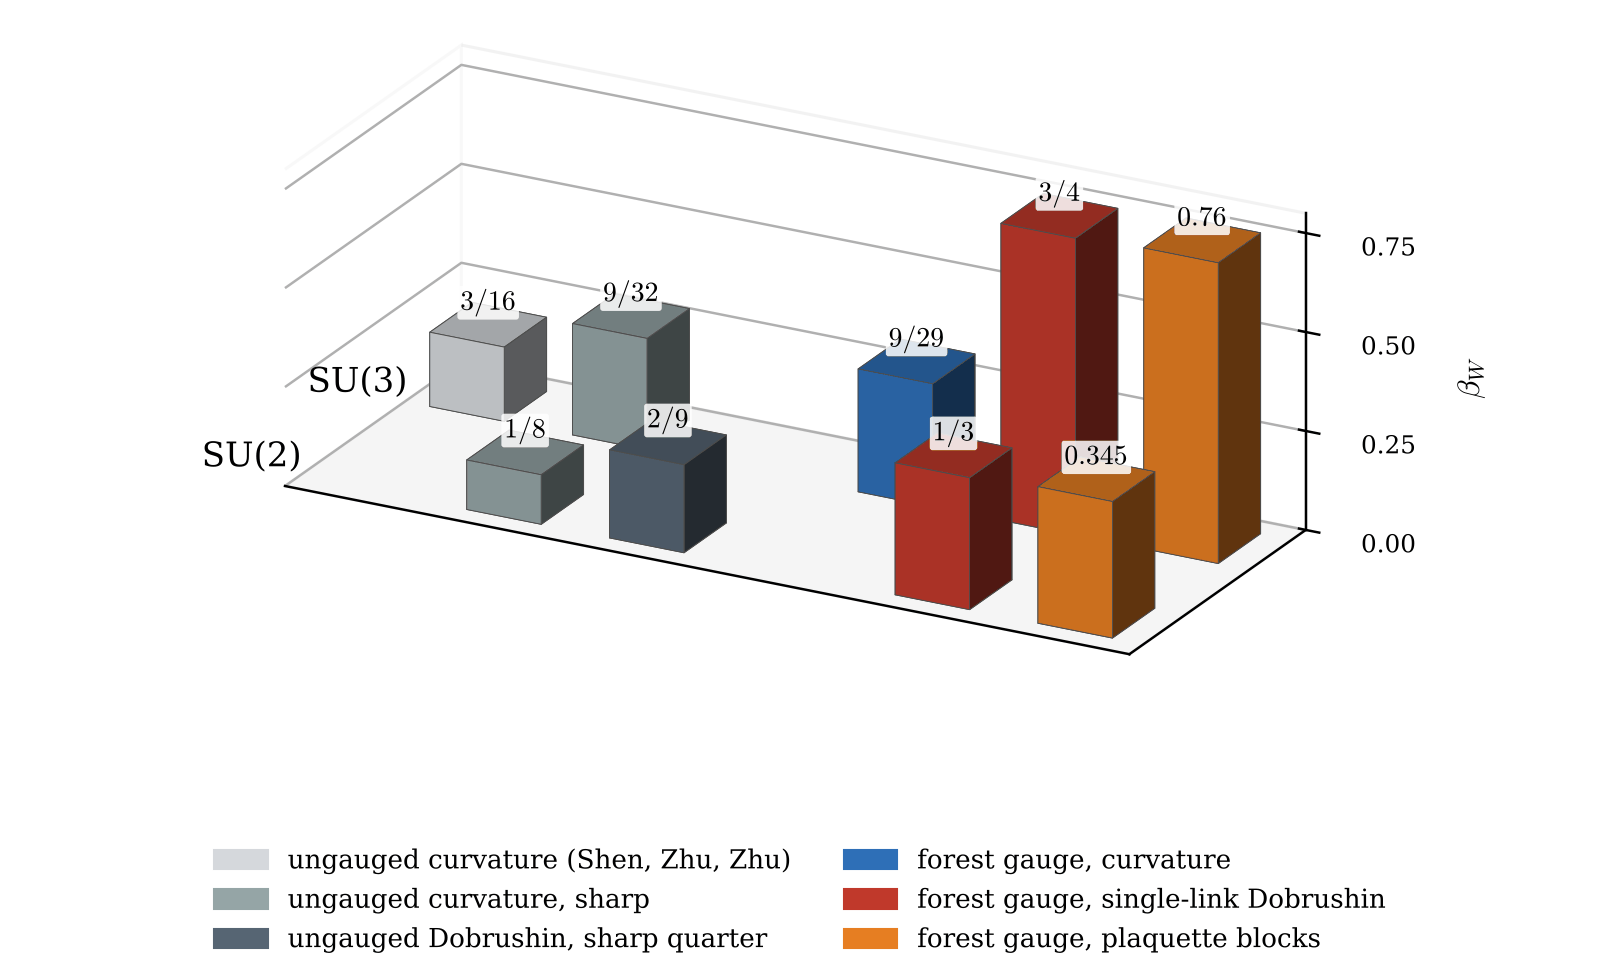
\includegraphics[width=\textwidth]{figures/fig_ranges.png}
\caption{Ranges of Table~\ref{tab:ranges}. The height of each bar is the
largest inverse coupling $\beta_W$ covered by the method. Grey bars are
methods for the ungauged measure; blue, red and orange bars use the forest
gauge. For $\SU(2)$ the red bar ends at the ceiling of
Theorem~\ref{thm:ceiling} and the orange bar, plaquette blocks, passes it
(Theorem~\ref{thm:blocks}); for $\SU(3)$ the red bar is
Theorem~\ref{thm:su3} and the orange bar, plaquette blocks, gives a larger
gap there and passes it (Theorem~\ref{thm:su3blocks}).}
\label{fig:ranges}
\end{figure}

All six theorems are statements at fixed lattice spacing. They do not touch
the continuum limit, the crossover to Ba{\l}aban's regime, or a gap in
physical units, which together are the Clay problem; Section~\ref{sec:limits}
says where each method stops and what remains of the four open problems
of~\cite{BB26a}. The obstruction proved in~\cite{BB26b}, that a lattice gap
uniform in lattice units forces trivial continuum two-point functions,
applies to all of them.

Section~\ref{sec:linefield} constructs the line field.
Section~\ref{sec:state} shows that a Dobrushin bound for the gauge-fixed
specification gives the full conclusion of Theorem~\ref{thm:su2}.
Sections~\ref{sec:su2}, \ref{sec:plaqblocks}, \ref{sec:curvature}
\ref{sec:su3} and~\ref{sec:su3blocks} prove Theorems~\ref{thm:su2}--\ref{thm:su3blocks}, and
Section~\ref{sec:limits} measures what is left. The appendices contain the
residue table of the line field, the comparison lemma and its version for
blocks, the blocks of the local Hessian inequality and the details of the
certified computation.

\section{The line field}\label{sec:linefield}

Write $e_0,\dots,e_3$ for the unit vectors of $\Z^4$ and $(x,\mu)$ for the
link from $x$ to $x+e_\mu$. A \emph{direction field} is a map
$\sigma:\Z^4\to\{0,1,2,3\}$; its links are $F=\{(x,\sigma(x)):x\in\Z^4\}$. At
each site put $\pi_x(\mu)=\sigma(x+e_\mu)$. The plaquette at $x$ in the plane
$\{\mu,\nu\}$ has the links $(x,\mu)$, $(x+e_\mu,\nu)$, $(x+e_\nu,\mu)$,
$(x,\nu)$, so it contains
\begin{equation}\label{eq:count}
[\sigma(x)\in\{\mu,\nu\}]+[\pi_x(\mu)=\nu]+[\pi_x(\nu)=\mu]
\end{equation}
links of $F$.

\begin{lemma}\label{lem:cycle}
Every plaquette of $\Z^4$ contains exactly one link of $F$ if and only if, at
every site $x$, $\pi_x$ fixes $\sigma(x)$ and permutes the other three
directions cyclically.
\end{lemma}

\begin{proof}
Fix $x$, let $s=\sigma(x)$ and let $R$ be the set of the other three
directions. For a plane $\{s,\nu\}$ the count~\eqref{eq:count} is $1+[\pi_x(s)
=\nu]+[\pi_x(\nu)=s]$; it equals one for all $\nu\in R$ exactly when
$\pi_x(s)=s$ and $\pi_x(\nu)\ne s$ for $\nu\in R$, that is, when $\pi_x$ fixes
$s$ and maps $R$ into $R$. For a plane $\{\mu,\nu\}\subset R$ the count is
$[\pi_x(\mu)=\nu]+[\pi_x(\nu)=\mu]$. Draw an arrow $\mu\to\pi_x(\mu)$ for every
$\mu\in R$ with $\pi_x(\mu)\in R\setminus\{\mu\}$. Each vertex of $R$ has at most
one outgoing arrow, and the condition says that each of the three pairs of
$R$ carries exactly one arrow. Three arrows on three vertices with out-degree
at most one give out-degree exactly one everywhere, and a tournament on three
vertices with all out-degrees one is a directed three-cycle.
\end{proof}

From now on $\sigma$ is the field of period two given in
Table~\ref{tab:sigma} of Appendix~\ref{app:table}, read from $x$ modulo two.
The table lists $\pi_x$ at each of the sixteen residue classes; in each row
$\pi_x$ fixes $\sigma(x)$ and is a three-cycle on the rest, so every plaquette
contains exactly one link of $F$ by Lemma~\ref{lem:cycle}.\footnote{There are
exactly eight period-two direction fields with this property, all equivalent
to $\sigma$ under the symmetries of the lattice. A field with one fixed link
at every site and one in every plaquette exists only in four dimensions: a
link lies in $2(d-1)$ plaquettes and a site carries $d(d-1)/2$ of them, and
$2(d-1)=d(d-1)/2$ forces $d=4$. The statements of this section are also
checked by \texttt{decide} in the Lean file \texttt{GaugeFix.lean} of the
archive.}

\begin{lemma}\label{lem:structure}
\begin{enumerate}[label=\textup{(\roman*)},leftmargin=*]
\item $F$ is a disjoint union of bi-infinite straight lines, one through
every site: every site has exactly one outgoing and one incoming link of $F$,
and both point in the direction $\sigma(x)$.
\item For every box $\Lambda$ (a product of four finite intervals, with the
links and plaquettes it contains), $F\cap E(\Lambda)$ is a disjoint union of
segments, hence a forest.
\item A link $e=(x,\mu)\notin F$ lies in six plaquettes. Four of them contain
a link of $F$ that shares an end point with $e$, and these lie in the planes
$\{\mu,\sigma(x)\}$ and $\{\mu,\pi_x(\mu)\}$. In the other two, which lie in
the remaining plane $\{\mu,\rho\}$, the link of $F$ is opposite to $e$.
\item Every link outside $F$ shares a plaquette with exactly twelve other
links outside $F$, two in each of its plaquettes.
\end{enumerate}
\end{lemma}

\begin{proof}
(i) Since $\pi_x$ fixes $\sigma(x)$, $\sigma(x+e_{\sigma(x)})=\sigma(x)$.
Because $\sigma$ has period two, $x-e_\mu\equiv x+e_\mu$, so also
$\sigma(x-e_{\sigma(x)})=\sigma(x)$, and the link $(x-e_{\sigma(x)},\sigma(x))$ is
in $F$. Conversely, if $(x-e_\nu,\nu)\in F$, then $\sigma(x-e_\nu)=\nu$, and
straightness at $x-e_\nu$ gives $\sigma(x)=\nu$. So the incoming link is unique
and continues the outgoing one.

(ii) A line meets a box in a segment, and distinct lines are disjoint.

(iii) The plaquettes of $e$ are, for each $\nu\ne\mu$, the one at $x$ and the
one at $x-e_\nu$ in the plane $\{\mu,\nu\}$. A link of $F$ sharing an end point
with $e$ is the outgoing or the incoming link of $F$ at $x$ or at $x+e_\mu$.
At $x$ both point in the direction $s=\sigma(x)\ne\mu$, and they lie in the
plaquettes at $x$ and at $x-e_s$ in the plane $\{\mu,s\}$. At $x+e_\mu$ both
point in the direction $t=\pi_x(\mu)$, which lies in $R\setminus\{\mu\}$ because
$\pi_x$ is a three-cycle on $R$, and they lie in the plaquettes at $x$ and at
$x-e_t$ in the plane $\{\mu,t\}$. These four plaquettes are distinct because
$s\ne t$. Each plaquette contains exactly one link of $F$, so in the two
plaquettes of the third plane $\{\mu,\rho\}$ the link of $F$ is a link of
direction $\mu$ or $\rho$ not touching $e$; the links of direction $\rho$ in
such a plaquette touch $e$, so it is the opposite link.

(iv) Each of the six plaquettes contains $e$, one link of $F$ and two other
links, and two distinct links share at most one plaquette.
\end{proof}

\begin{figure}[tb]
\centering
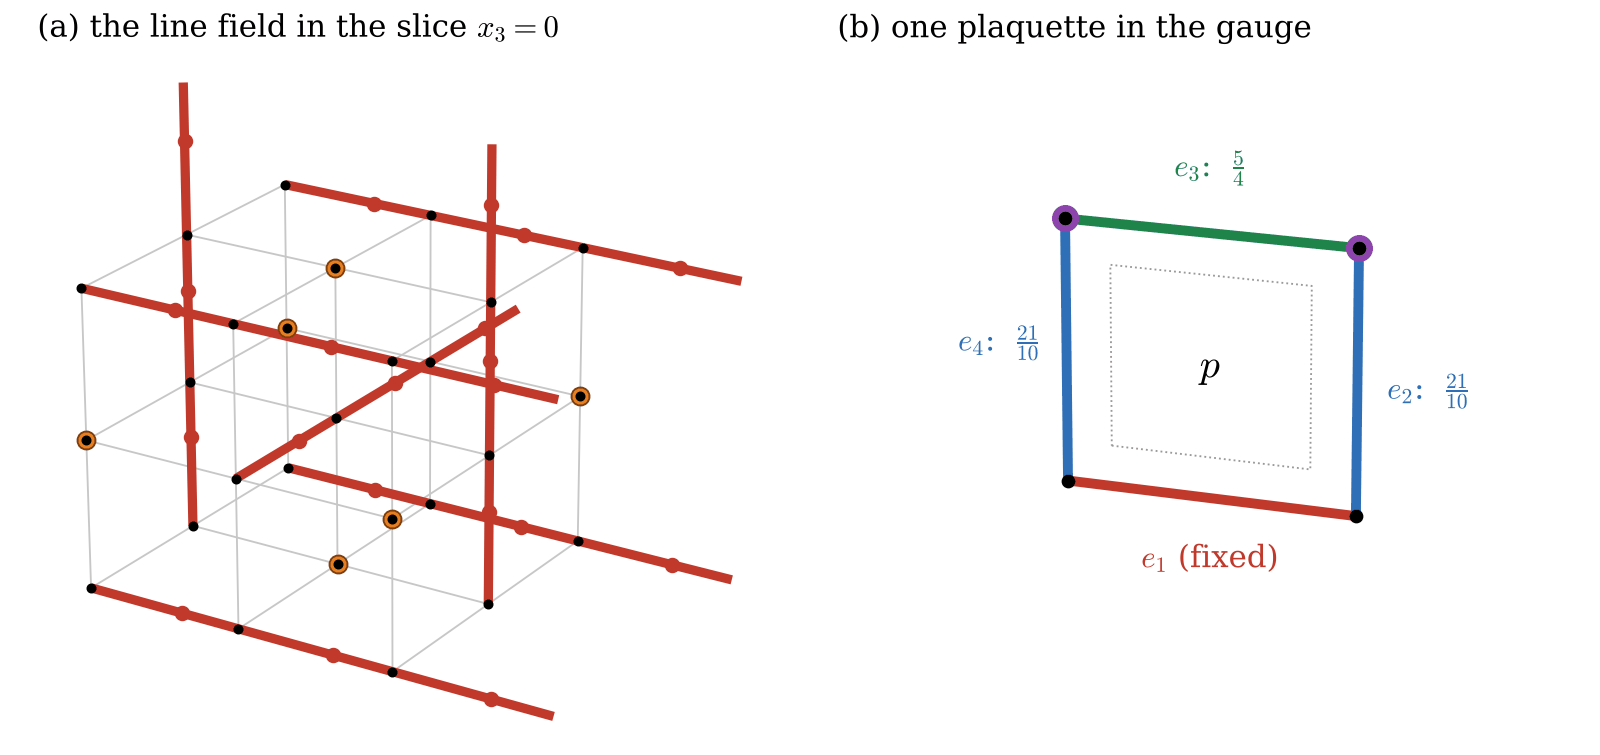
\includegraphics[width=\textwidth]{figures/fig_linefield.png}
\caption{(a) The line field in the slice $x_3=0$ of a box of side three.
Thick red segments are the links of $F$ in the directions $0,1,2$, with a dot
marking the direction of travel; an orange ring marks a site whose line
leaves the slice in direction~$3$. Every line is straight
(Lemma~\ref{lem:structure}(i)), and the segments that leave the box are its
boundary stubs. (b) One plaquette with its fixed link $e_1$. The weights are
those of the local inequality of Lemma~\ref{lem:local} for the three free
links: $\frac{21}{10}$ on the two links adjacent to $e_1$ and $\frac54$ on the
opposite one. The two purple corners are the ones that enter the corner
form~\eqref{eq:corner} once $Y_1=0$.}
\label{fig:linefield}
\end{figure}

\section{Gauge fixing and the free-boundary state}\label{sec:state}

Let $G\subset\U(N)$ be compact with Haar measure $dU$, and let $\Lambda$ be a
box. The Wilson measure with free boundary is
\[
W_\Lambda(dQ)=\frac1{Z_\Lambda}\exp\Bigl(N\beta\sum_{p\in P(\Lambda)}\ReTr
Q_p\Bigr)\prod_{e\in E(\Lambda)}dQ_e .
\]
The measure is invariant under the gauge transformations $Q_{(x,y)}\mapsto
g_xQ_{(x,y)}g_y^{-1}$ with $g\in G^\Lambda$. Call the links outside $F$ \emph{active} and
write $A$ for their set. For a function $O$ of the links, $O^F$ is $O$ with
every link of $F$ set to the identity.

\begin{lemma}[Gauge fixing]\label{lem:gaugefix}
Let $\mu^F_\Lambda$ be the probability measure on $G^{A\cap E(\Lambda)}$
whose density with respect to Haar measure is proportional to
$\exp(N\beta\sum_{p\in P(\Lambda)}\ReTr Q^F_p)$. For every gauge-invariant $O$ on $G^{E(\Lambda)}$,
\[
W_\Lambda(O)=\mu^F_\Lambda(O^F).
\]
\end{lemma}

\begin{proof}
Each segment of $F\cap E(\Lambda)$ is a path $x_0,x_1,\dots,x_k$ along one
direction. Given the variables on $F$, put $g_{x_0}=1$ and $g_{x_{i+1}}=
g_{x_i}Q_{(x_i,x_{i+1})}$ on every segment. The transformed field has $Q^g_e
=1$ on $F\cap E(\Lambda)$, and for fixed values on $F$ the map $Q_A\mapsto
Q^g_A$ is a product of left and right translations, which preserves Haar
measure. Gauge invariance of the action and of $O$ and the change of
variables give the claim.
\end{proof}

No leftover holonomy appears because $F\cap E(\Lambda)$ is a forest. The
measures $\mu^F_\Lambda$ are finite-volume versions of the specification
$\gamma^F$ on $G^A$: for $e\in A$, $\gamma^F_e$ resamples $Q_e$ from the law
with density proportional to $\exp(N\beta\sum_{p\ni e}\ReTr Q^F_p)$ given all
other active links. No infinite-volume gauge transformation is performed;
$\gamma^F$ is a specification in its own right. Fix a metric $\delta$ on $G$
of diameter $D$ that is bi-invariant (for $\SU(2)$ the chordal metric on
$S^3$, $D=2$; for $\SU(N)$ the Hilbert--Schmidt distance). The Kantorovich
coefficient of $e'$ on $e$ is
\[
C_{ee'}=\sup\frac{W_1\bigl(\gamma^F_e(\cdot\mid Q),\gamma^F_e(\cdot\mid
Q')\bigr)}{\delta(Q_{e'},Q'_{e'})},
\]
the supremum over pairs of configurations that differ only at $e'$. It
vanishes unless $e$ and $e'$ share a plaquette.

\begin{proposition}\label{prop:state}
Suppose that every row and every column of $(C_{ee'})$ sums to at most
$\alpha<1$. Then:
\begin{enumerate}[label=\textup{(\roman*)},leftmargin=*]
\item $\gamma^F$ has exactly one Gibbs measure $\mu_F$;
\item for every gauge-invariant local $O$ the limit $\omega(O)=\lim
W_\Lambda(O)$ exists along every sequence of boxes exhausting $\Z^4$ and
equals $\mu_F(O^F)$;
\item $\omega$ is invariant under translations and the hypercubic group;
\item if $\beta\ge0$, $\omega$ is reflection positive for reflections in
hyperplanes through sites and in hyperplanes bisecting links;
\item for gauge-invariant local $O,O'$ with $O$ Lipschitz in each link,
$|\Cov_\omega(O,O')|\le C_{O,O'}e^{-\lambda\dist(O,O')}$ for every
$\lambda<-\log\alpha$;
\item if $\beta\ge0$, the transfer matrix of $\omega$ has spectral gap at
least $-\log\alpha$.
\end{enumerate}
\end{proposition}

\begin{proof}
(i) Gibbs measures exist by compactness, and the comparison lemma of
Appendix~\ref{app:comparison} with $S=\emptyset$ shows that any two coincide.

(ii) Extend $\mu^F_\Lambda$ by Haar measure on the active links outside
$\Lambda$, and let $S$ be the set of active links with a plaquette outside
$P(\Lambda)$; this includes every active link outside $E(\Lambda)$. For an
active link $e\notin S$ all six plaquettes of $e$ lie in $P(\Lambda)$, so the
conditional law of $Q_e$ under the extended measure is $\gamma^F_e$. Let $T$
be the support of $O^F$ and $\lambda<-\log\alpha$. The comparison lemma with
weights $e^{-\lambda\dist(\cdot,T)}$ gives
\[
|\mu^F_\Lambda(O^F)-\mu_F(O^F)|\le L\,\frac{\theta D}{1-\theta}
\sum_{z\in S}e^{-\lambda\dist(z,T)},
\]
with $\theta=\alpha e^\lambda<1$ and $L$ a Lipschitz constant of $O^F$; the
sum is at most $C_TR^3e^{-\lambda R}$ when $R$ is the distance from $T$ to the
complement of $\Lambda$. For $O$ continuous but not Lipschitz, approximate
uniformly. Lemma~\ref{lem:gaugefix} gives $W_\Lambda(O)=\mu^F_\Lambda(O^F)$.

(iii) $W_\Lambda(\tau_vO)=W_{\Lambda-v}(O)$, and the boxes $\Lambda-v$ also
exhaust $\Z^4$; by (ii) the limit does not depend on the sequence. The line
field is a device for computing $W_\Lambda$ and is never shifted. The same
argument applies to the hypercubic group.

(iv) For $\beta\ge0$ the measure $W_\Lambda$ is reflection positive for every
box symmetric under the reflection~\cite{OSei78}, and reflection positivity
passes to the limit along such boxes, which is $\omega$ by (ii).

(v) $\Cov_\omega(O,O')=\Cov_{\mu_F}(O^F,O'^F)$, and setting the links of $F$
to the identity keeps the Lipschitz property. The bound is
Corollary~\ref{cor:decay}.

(vi) Let $\vartheta$ be a time reflection and $\tau_t$ a time translation.
For gauge-invariant local $O$ that are Lipschitz in each link, (v) gives
$|\omega(\vartheta(\bar O)\tau_tO)-|\omega(O)|^2|\le C_Oe^{-\lambda t}$. On
the support of $O$ these functions are dense in the gauge-invariant part of
$L^2(\omega)$: gauge-invariant functions are functions on the compact
quotient of $G^{E}$ by the gauge group, Lipschitz functions for the quotient
metric are dense in $L^2$ of every finite measure on it, and they lift to
gauge-invariant Lipschitz functions. By~\cite[Prop.~23]{BB26a} the spectrum
of the transfer matrix on the complement of the vacuum lies in
$[0,e^{-\lambda}]$, for every $\lambda<-\log\alpha$.
\end{proof}

The proposition replaces the torus limits and the uniqueness of the
ungauged Gibbs measure used in~\cite[Thm.~F]{BB26a} by the free-boundary
limit, which has all the properties the reconstruction of the transfer
matrix needs.\footnote{On a torus the line field closes up into cycles, and
the holonomies along them cannot be removed by a gauge transformation; the
argument never uses a torus. The state $\omega$ is defined only on
gauge-invariant observables, which is all that the Osterwalder--Schrader
reconstruction~\cite{OS73,OS75,OSei78} uses.}

\section{SU(2) up to one third}\label{sec:su2}

\begin{proof}[Proof of Theorem~\ref{thm:su2}]
Identify $\SU(2)$ with the unit quaternions and use the chordal metric. For an
active link $e$ and a plaquette $p\ni e$, the staple $s_p$ is the product of the
other three link variables in the order that makes $\operatorname{Re}(Q_es_p)
=\frac12\Tr Q_p$, with links of $F$ equal to one. Since $N\beta\ReTr Q_p=
4\beta\ip{Q_e}{\bar s_p}$ in $\R^4$, the conditional law of $Q_e$ is the von
Mises--Fisher law $\nu_b(dx)\propto e^{\ip xb}dx$ on $S^3$ with $b=4\beta
\sum_{p\ni e}\bar s_p$. Changing a partner $e'$ by $\delta$ in the chordal
metric changes one staple by an isometric image of that displacement, so $b$
moves by $4|\beta|\delta$, and the sharp quarter~\cite[Thm.~7]{BB26a},
$W_1(\nu_b,\nu_{b'})\le\frac14|b-b'|$, gives $C_{ee'}\le|\beta|$. By
Lemma~\ref{lem:structure}(iv) every row and column has twelve nonzero
entries, so $\alpha\le12|\beta|=3|\beta_W|$. Proposition~\ref{prop:state}
applies for $|\beta_W|<\frac13$.
\end{proof}

\begin{proof}[Proof of Theorem~\ref{thm:ceiling}]
For the line field, every staple of an active link contains two active
links, so the six staples can be chosen with sum zero while the staple
through a given partner $e'$ moves freely. At $b=0$ the derivative of $\nu_b$
in the direction $h$ has Kantorovich norm $\frac14|h|$~\cite[Lemma~6(i)]{BB26a},
so $C_{ee'}=|\beta|$ exactly, and every row sum is $12|\beta|=3|\beta_W|$.

Now let $F'$ be any forest and $C'$ the matrix of the statement. Suppose a
positive weight $w$ satisfies $C'w\le\alpha w$. For a box $\Lambda_n$ of side
$n$ let $C_n$ be the principal submatrix on the active links of $E(\Lambda_n)$;
then $C_nw\le\alpha w$ on these links, and the Collatz--Wielandt inequality
for nonnegative matrices gives $\rho(C_n)\le\alpha$. Since $C_n$ is symmetric,
$\rho(C_n)$ is at least the mean row sum. The box has $4n^4-O(n^3)$ links and
$n^4$ sites, and a forest has fewer links than sites, so the number $a$ of
active links is at least $3n^4-O(n^3)$. Let $a_p$ be the number of active
links of the plaquette $p$; the box has $P=6n^4-O(n^3)$ plaquettes and
$\sum_pa_p=6a-O(n^3)$. Two links share at most one plaquette, so the row
sums add up to $|\beta|\sum_pa_p(a_p-1)$, and by convexity
\[
\frac{|\beta|}a\sum_pa_p(a_p-1)\ge\frac{|\beta|P}a\,\bar a(\bar a-1)
=6|\beta|(\bar a-1)-o(1),
\]
with $\bar a=\sum_pa_p/P=6a/P-o(1)\ge3-o(1)$. Hence $\alpha\ge12|\beta|-o(1)$
for every $n$, and $\alpha\ge12|\beta|=3|\beta_W|$.
\end{proof}

Without gauge fixing the same count gives eighteen partners and the ceiling
$\beta_W=\frac29$ of~\cite[Prop.~13]{BB26a}; the temporal gauge, a family of
lines in one direction, leaves fourteen. The line field is optimal among
forests: twelve is the mean number of partners forced by the number of free
links, and it is attained at every link.

\section{SU(2) past one third: plaquette blocks}\label{sec:plaqblocks}

Throughout this section $G=\SU(2)$ is the group of unit quaternions with
the chordal metric $|x-y|$, $\bar x$ is the conjugate, $\ip xy=\operatorname{Re}
(x\bar y)$ is the inner product of $\R^4$, and $dx$ is the normalised Haar
measure on $S^3$. Left and right multiplication by unit quaternions and
conjugation are isometries, and $\operatorname{Re}(xyz)=\operatorname{Re}
(yzx)=\ip y{\bar z\bar x}$. Put
\[
Z_0(c)=\int_{S^3}e^{\ip cx}dx=\sum_{j\ge0}\frac{(|c|^2/4)^j}{j!\,(j+1)!},
\qquad c\in\R^4,
\]
let $\nu_c(dx)\propto e^{\ip cx}dx$ be the von Mises--Fisher law, and write
$g=\log Z_0$, so that $\nabla g(c)$ is the mean and $\Hess g(c)$ the
covariance of $\nu_c$.

\subsection{The blocks}

A \emph{block plaquette} is a plaquette of the set $\mathcal B$ described in
Table~\ref{tab:plaqblocks} of Appendix~\ref{app:plaqblocks}, and its
\emph{block} is the set of its three active links.

\begin{lemma}\label{lem:plaqblocks}
The set $\mathcal B$ is invariant under translations by $2\Z^4$ and:
\begin{enumerate}[label=\textup{(\roman*)},leftmargin=*]
\item the blocks partition the active links;
\item every plaquette $p\notin\mathcal B$ meets three distinct blocks, one in
each of its active links;
\item every active link lies in exactly five plaquettes outside $\mathcal B$,
so it shares a plaquette outside $\mathcal B$ with exactly ten active links,
none of them in its own block;
\item if an active link $j$ and a link of a block $B$ lie in a common
plaquette outside $\mathcal B$, then every link of $B$ has its midpoint
within distance $2$ of the midpoint of $j$.
\end{enumerate}
\end{lemma}

\begin{proof}
All four statements are invariant under $2\Z^4$ and involve plaquettes at
distance at most two from one site, so they hold on $\Z^4$ as soon as they
hold on the torus $(\Z/P\Z)^4$ with $P\ge6$, where no such configuration
wraps around. They are checked on the tori of side four and six by the
program described in Appendix~\ref{app:plaqblocks}; the side four already
suffices for (i)--(iii). For (iii), an active link lies in six plaquettes,
one of which is its block plaquette, and each of the other five contains two
further active links, which lie in other blocks by (ii).
\end{proof}

Fix a block plaquette $p$ with active links $e_1,e_2,e_3$. Reading the
plaquette product cyclically and deleting its fixed link, $\frac12\Tr Q_p=
\operatorname{Re}(y_1y_2y_3)$, where $y_i$ is $Q_{e_i}$ or $Q_{e_i}^{-1}$.
Every other plaquette containing $e_i$ meets the block only in $e_i$ by
Lemma~\ref{lem:plaqblocks}(ii) and contributes $4\beta\ip{y_i}{\bar s}$ to
the exponent, where $s$ is the staple of $y_i$ in it. Hence the conditional
law of the block given all other active links is
\begin{equation}\label{eq:blocklaw}
\mu_b(dy)\propto\exp\Bigl(\sum_{i=1}^3\ip{y_i}{b_i}+4\beta\operatorname{Re}
(y_1y_2y_3)\Bigr)dy_1\,dy_2\,dy_3,
\end{equation}
with $b_i$ the sum of $4\beta\bar s$ over the five staples, so that
$|b_i|\le20|\beta|$. Inversion is an isometry of $S^3$ and preserves Haar
measure, so we may work with $y$ instead of $Q$. On $(S^3)^3$ we use the
metric $d(y,y')=\sum_i|y_i-y'_i|$.

\subsection{The sensitivity of one block}

Let $\lambda_*$ and $\tau$ be a lower and an upper bound for the
eigenvalues of $\Hess g(c)$ on the ball $|c|\le24|\beta|$, and $M$ an upper
bound there for the norm of the third derivative $D^3g(c)$ as a trilinear
form. Put
\begin{equation}\label{eq:blockconst}
\begin{gathered}
w=8\beta^2(\tau-\lambda_*),\qquad s=\tfrac14+(e^w-1)e^w\sqrt\tau,\\
C=20|\beta|\bigl(4|\beta|\tau s+16\beta^2M\bigr),\qquad
K=\frac{(1+|\beta|)\,s}{1-C},
\end{gathered}
\end{equation}
assuming $C<1$.

\begin{lemma}\label{lem:tilt}
Let $\nu$ be a probability measure and $\lambda=e^R\nu/\nu(e^R)$ with
$\operatorname{osc}R\le\omega$. For bounded $f,h$,
\[
\Cov_\lambda(f,h)\le\Cov_\nu(f,h)+(e^\omega-1)e^\omega\,\mathrm{sd}_\nu(f)
\,\mathrm{sd}_\nu(h).
\]
\end{lemma}

\begin{proof}
We may assume $0\le R\le\omega$. The density $\rho=e^R/\nu(e^R)$ lies in
$[e^{-\omega},e^\omega]$, so $\delta=\|\rho-1\|_\infty\le e^\omega-1$. With
$\tilde f=f-\nu f$ and $\tilde h=h-\nu h$,
\[
\begin{split}
\Cov_\lambda(f,h)-\Cov_\nu(f,h)={}&\nu\bigl((\rho-1)\tilde f\tilde h\bigr)\\
&-\nu\bigl((\rho-1)\tilde f\bigr)\,\nu\bigl((\rho-1)\tilde h\bigr),
\end{split}
\]
and the right side is at most $(\delta+\delta^2)\,\mathrm{sd}_\nu(f)\,
\mathrm{sd}_\nu(h)$ by the Cauchy--Schwarz inequality.
\end{proof}

\begin{lemma}\label{lem:onesite}
Let $\beta\ge0$, $a,c_0\in\R^4$ with $|a|,|c_0|\le20\beta$, and
\[
\kappa(dx)\propto\exp\bigl(\ip xa+g(c_0+4\beta\bar x)\bigr)dx
\quad\text{on }S^3 .
\]
For every $1$-Lipschitz $f$ and every $h\in\R^4$:
\begin{enumerate}[label=\textup{(\roman*)},leftmargin=*]
\item $\Cov_\kappa(f,\ip xh)\le s|h|$;
\item if $c_0$ moves in the direction $k$, then $|\frac{d}{dt}\kappa(f)|\le
(4\beta\tau s+16\beta^2M)|k|$.
\end{enumerate}
\end{lemma}

\begin{proof}
(i) Taylor's formula at $c_0$ gives $g(c_0+4\beta u)=g(c_0)+4\beta\ip{\nabla
g(c_0)}u+R(u)$ with $R(u)=8\beta^2\Hess g(\xi)(u,u)$ for some $\xi$ on the
segment, $|\xi|\le24\beta$. For $u=\bar x$ of norm one, $R(\bar x)\in[8\beta^2
\lambda_*,8\beta^2\tau]$, so $\operatorname{osc}R\le w$. Since $\ip{\nabla
g(c_0)}{\bar x}=\ip x{\overline{\nabla g(c_0)}}$, $\kappa$ is the tilt
$e^{R}\nu/\nu(e^R)$ of $\nu=\nu_c$ with $c=a+4\beta\overline{\nabla g(c_0)}$.
The sharp quarter~\cite[Thm.~7]{BB26a} gives $\Cov_\nu(f,\ip xh)=\frac{d}{dt}
\nu_{c+th}(f)\le\frac14|h|$. A $1$-Lipschitz function on a set of diameter
two has $\mathrm{sd}\le1$, and $\mathrm{sd}_\nu\ip xh\le\sqrt\tau|h|$
because $|c|\le|a|+4\beta\le24\beta$. Lemma~\ref{lem:tilt} gives (i).

(ii) The derivative is $\Cov_\kappa(f,\ip{\nabla g(c_0+4\beta\bar x)}k)$.
Write $\nabla g(c_0+4\beta u)=\nabla g(c_0)+4\beta\Hess g(c_0)u+N(u)$. The
constant term does not contribute. The linear term is $\ip xh$ with
$h=4\beta\,\overline{\Hess g(c_0)k}$, $|h|\le4\beta\tau|k|$, and contributes at
most $4\beta\tau s|k|$ by (i). For $|u|,|u'|\le1$, $\|\Hess g(c_0+4\beta v)-
\Hess g(c_0)\|\le4\beta M|v|\le4\beta M$ on the segment between them, so
$|N(u)-N(u')|\le16\beta^2M|u-u'|$; the function $\ip{N(\bar x)}k$ is
therefore $16\beta^2M|k|$-Lipschitz, its standard deviation is at most that
constant, and its covariance with $f$ is at most $16\beta^2M|k|$.
\end{proof}

\begin{lemma}\label{lem:blockK}
Let $C<1$. If $b$ and $b'$ satisfy $|b_i|,|b'_i|\le20|\beta|$ and differ
only in one coordinate $b_i$, then
\[
W_1(\mu_b,\mu_{b'})\le K\,|b_i-b'_i|
\]
in the metric $d$.
\end{lemma}

\begin{proof}
The map $y_1\mapsto-y_1$ turns $\mu_b$ for $\beta$ into the law for $-\beta$
with $b_1$ replaced by $-b_1$ and is an isometry, so we may take $\beta\ge0$;
the cyclic symmetry of $\operatorname{Re}(y_1y_2y_3)$ lets us take $i=1$. Let
$f$ be $1$-Lipschitz for $d$ and $\varepsilon=|b_1-b'_1|$.

\emph{The middle link.} Given $y_1,y_3$, the law of $y_2$ is $\nu_c$ with $c=
b_2+4\beta\,\overline{y_3y_1}$, which does not involve $b_1$. Changing $y_1$
by $\eta$ moves $c$ by $4\beta\eta$, and the sharp quarter moves $\nu_c$ by at
most $\beta\eta$ in $W_1$. Hence $F(y_1,y_3)=\E[f\mid y_1,y_3]$ is
$(1+\beta)$-Lipschitz in each variable, and $\mu_b(f)=\mu^{13}_b(F)$, where
$\mu^{13}_b$ is the law of $(y_1,y_3)$:
\[
\mu^{13}_b\propto e^{\ip{y_1}{b_1}+\ip{y_3}{b_3}}Z_0\bigl(b_2+4\beta\,
\overline{y_3y_1}\bigr).
\]
Since $|b_2+4\beta\overline{y_3y_1}|=|b_2y_3+4\beta\bar y_1|=|y_1b_2+
4\beta\bar y_3|$, its conditional laws are
\[
\begin{split}
\kappa_1(dy_1\mid y_3)&\propto e^{\ip{y_1}{b_1}+g(b_2y_3+4\beta\bar y_1)}dy_1,\\
\kappa_3(dy_3\mid y_1)&\propto e^{\ip{y_3}{b_3}+g(y_1b_2+4\beta\bar y_3)}dy_3,
\end{split}
\]
both of the form of Lemma~\ref{lem:onesite}, with $|c_0|=|b_2|$.

\emph{Two sites.} Integrating Lemma~\ref{lem:onesite}(i) along the segment
from $b_1$ to $b'_1$ gives $W_1(\kappa_1,\kappa'_1)\le s\varepsilon$ for the
same $y_3$. Moving $y_3$ to $y'_3$ moves $c_0=b_2y_3$ along a segment of
length $|b_2||y_3-y'_3|\le20\beta|y_3-y'_3|$ inside the ball $|c_0|\le20\beta$,
so Lemma~\ref{lem:onesite}(ii) gives $W_1(\kappa_1(\cdot\mid y_3),\kappa_1(
\cdot\mid y'_3))\le C|y_3-y'_3|$, and the same for $\kappa_3$, which does not
depend on $b_1$. Let $\pi$ be a coupling of $\mu^{13}_b$ and $\mu^{13}_{b'}$
minimising $d_1+d_3$, $d_k=\E_\pi|y_k-y'_k|$. Replacing $(y_1,y'_1)$ by an
optimal coupling of $\kappa_1(\cdot\mid y_3)$ and $\kappa'_1(\cdot\mid y'_3)$
keeps a coupling, so minimality gives $d_1\le s\varepsilon+Cd_3$; in the
same way $d_3\le Cd_1$. Hence $d_1\le s\varepsilon/(1-C^2)$ and
\[
|\mu_b(f)-\mu_{b'}(f)|\le(1+\beta)(d_1+d_3)\le\frac{(1+\beta)s}{1-C}
\,\varepsilon=K\varepsilon .\qedhere
\]
\end{proof}

\subsection{The constants}

\begin{lemma}\label{lem:vmfconst}
Write $g(c)=\varphi(|c|^2)$ and $r=|c|$. For $c\ne0$ the eigenvalues of
$\Hess g(c)$ are $2\varphi'(r^2)$, three times, and $2\varphi'(r^2)+4r^2
\varphi''(r^2)$, and the norm of $D^3g(c)$ is
\[
\max\Bigl(|A+\Gamma|,\tfrac23|A|\Bigr),\qquad A=12r\varphi''(r^2),\quad
\Gamma=8r^3\varphi'''(r^2).
\]
On the ball $r\le2.07$ every eigenvalue of $\Hess g$ lies between
$0.158491$ and $0.25000001$, and the norm of $D^3g$ is at most $0.0615586$.
\end{lemma}

\begin{proof}
Differentiating $\varphi(|c|^2)$ gives $D^2g(v,v)=2\varphi'|v|^2+4\varphi''
\ip cv^2$ and $D^3g(v,v,v)=12\varphi''\ip cv|v|^2+8\varphi'''\ip cv^3$. For
$|v|=1$ and $t=\ip{c/r}v\in[-1,1]$ the cubic form is $At+\Gamma t^3$, whose
largest absolute value is attained at $t=\pm1$ or at an interior critical
point, where it equals $\frac23|A||t|\le\frac23|A|$; by Banach's
theorem~\cite{Ban38} the supremum of a symmetric trilinear form on the
diagonal of the unit sphere is its norm. The numerical bounds are obtained
in ball arithmetic~\cite{Joh17} from the series of $Z_0$, truncated after
forty terms with a proved bound on the tail, on $2\cdot10^4$ subintervals of
$[0,2.07]$; the program is described in Appendix~\ref{app:plaqblocks}.
\end{proof}

\subsection{The proof of Theorem~\ref{thm:blocks}}

Let $\gamma^{\mathcal B}$ be the block specification: for a block $B$,
$\gamma^{\mathcal B}_B$ resamples the three links of $B$ from~\eqref{eq:blocklaw}.
It comes from the same interaction as $\gamma^F$, so the two specifications
have the same Gibbs measures. Define the block coefficients
\[
C_{Bj}=\sup\frac{W_1\bigl(\gamma^{\mathcal B}_B(\cdot\mid Q),\gamma^{\mathcal B}_B
(\cdot\mid Q')\bigr)}{|Q_j-Q'_j|}
\]
for an active link $j\notin B$, the supremum over pairs of configurations
that differ only at $j$, with $W_1$ for the metric $d$.

\begin{proposition}\label{prop:blockstate}
Suppose that $\sum_BC_{Bj}\le\alpha<1$ for every active link $j$. Then the
conclusions (i)--(vi) of Proposition~\ref{prop:state} hold with
$-\frac12\log\alpha$ in place of $-\log\alpha$.
\end{proposition}

\begin{proof}
The proof of Proposition~\ref{prop:state} goes through with
Lemma~\ref{lem:blockcomparison} of Appendix~\ref{app:comparison} in place of
Lemma~\ref{lem:comparison}, and with the set $S$ of part~(ii), and the
support of $H$ in Corollary~\ref{cor:decay}, enlarged to the union of the
blocks that meet it. The enlargement multiplies the size of these sets by at
most three and moves them by at most one, which changes only the constants.
\end{proof}

\begin{proof}[Proof of Theorem~\ref{thm:blocks}]
Let $|\beta|\le0.345/4$ and take the constants of Lemma~\ref{lem:vmfconst},
whose ball $r\le2.07$ contains $|c|\le24|\beta|$. With these fixed constants
every quantity in~\eqref{eq:blockconst} is increasing in $|\beta|$, and so is
\begin{equation}\label{eq:alphablock}
\alpha(\beta_W)=40|\beta|K .
\end{equation}
Changing an active link $j$ by $\eta$ changes one staple of each of its ten
partners outside its block by an isometric image of the displacement, so the
field $b_i$ of each such partner $i$ moves by at most $4|\beta|\eta$, and
Lemma~\ref{lem:blockK}, applied once for each of these ten fields, gives
$\sum_BC_{Bj}\le40|\beta|K$. Evaluating~\eqref{eq:blockconst} in ball
arithmetic at $\beta_W=0.345$ gives $w\le0.0054459$, $s\le0.252746$,
$C\le0.050243$, $K\le0.289069$ and $\alpha\le0.99729$; at $\beta_W=\frac13$ it
gives $\alpha\le0.95602$. Proposition~\ref{prop:blockstate} applies.
\end{proof}

\begin{remark}\label{rem:blockgap}
Most of the range is kept. A second bound for the same sensitivity, which
keeps the law of the middle link instead of linearising it, evaluated in
floating point on a quadrature grid and maximised over the fields $b$ by a
random search followed by the Nelder--Mead method, gives $0.2783$ at
$\beta_W=0.34$, against $0.2881$ from Lemma~\ref{lem:blockK}, and $40|\beta|$
times it crosses one near $\beta_W=0.357$. That computation is not certified
and is not used in the proof. Past this point the gain from integrating out
one link is spent, and larger blocks are needed, such as the free links of a
cube of the line field, whose sensitivity no longer reduces to two sites.
\end{remark}

\section{Curvature in the gauge}\label{sec:curvature}

In this section $G=\SU(N)$, $\SO(N)$ or $\U(N)$ with the inner product
$\ip XY=-\Tr(XY)$ on the Lie algebra, so that $\Ric_{\SU(N)}=\frac N2$ and
$\Ric_{\SO(N)}=\frac{N-2}4$. A tangent vector at a field $Q$ is $v=(X_eQ_e)$,
$|v|^2=\sum_e|X_e|^2$. For the plaquette at $x$ in the plane $\mu<\nu$ number
its links $e_1=(x,\mu)$, $e_2=(x+e_\mu,\nu)$, $e_3=(x+e_\nu,\mu)$,
$e_4=(x,\nu)$, transport their vectors to $x$,
\begin{equation}\label{eq:transport}
Y_1=X_{e_1},\ \ Y_2=Q_{e_1}X_{e_2}Q_{e_1}^*,\ \
Y_3=Q_{e_4}X_{e_3}Q_{e_4}^*,\ \ Y_4=X_{e_4},
\end{equation}
and write $W=Q_p$. The second derivative of $\ReTr Q_p$ along the geodesic
$Q_e(t)=e^{tX_e}Q_e$ is~\cite[Eq.~(5)]{BB26a}
\begin{equation}\label{eq:fp}
\begin{split}
f_p={}&\sum_{i=1}^4\ReTr(Y_i^2W)+2\ReTr(Y_1Y_2W)+2\ReTr(Y_3Y_4W)\\
&-2\sum_{i\in\{1,2\},\,j\in\{3,4\}}\ReTr(Y_iWY_j),
\end{split}
\end{equation}
so that $\Hess S_0(v,v)=\sum_pf_p$. The corner form of $p$ is
\begin{equation}\label{eq:corner}
c_p=2\ip{Y_1}{Y_4}-2\ip{Y_1}{Y_2}+2\ip{Y_2}{WY_3W^*}-2\ip{Y_3}{Y_4}.
\end{equation}
It collects the inner products of the transported vectors of two links that
meet at a right angle at a corner of $p$.

\begin{lemma}\label{lem:identity}
On $\Z^4$, or on a box with free boundary, for every field $Q$ and every
square-summable $X$,
\[
\begin{split}
&\sum_y\Bigl[|D_yX|^2+\sum_\mu\bigl|X_{y,\mu}+Q^*_{y-e_\mu,\mu}X_{y-e_\mu,\mu}
Q_{y-e_\mu,\mu}\bigr|^2\Bigr]\\
&\qquad=4|X|^2+\sum_pc_p ,
\end{split}
\]
where $D_yX=\sum_\mu[X_{y,\mu}-Q^*_{y-e_\mu,\mu}X_{y-e_\mu,\mu}Q_{y-e_\mu,\mu}]$ is
the covariant divergence and terms with a link outside the box are omitted.
\end{lemma}

\begin{proof}
At a site $y$ write $o_\mu$ for the vector of the outgoing link in direction
$\mu$ and $i_\mu$ for the transported vector of the incoming one, so that
$D_yX=\sum_\mu(o_\mu-i_\mu)$. Every link is outgoing at one end and incoming at
the other, so the squares $|o_\mu|^2+|i_\mu|^2$, which appear once in
$|D_yX|^2$ and once in $|o_\mu+i_\mu|^2$, add up to $4|X|^2$. The collinear
cross term $-2\ip{o_\mu}{i_\mu}$ of $|D_yX|^2$ cancels the term
$+2\ip{o_\mu}{i_\mu}$ of $|o_\mu+i_\mu|^2$. The remaining cross terms of
$|D_yX|^2$ pair two perpendicular ends at $y$, and each such pair is a corner
of exactly one plaquette, with the sign and the transport of~\eqref{eq:corner}
(this is the proof of~\cite[Lemma~1]{BB26a}). In a box two perpendicular ends at $y$ span
a plaquette of the box, because a box is a product of intervals.
\end{proof}

\begin{lemma}\label{lem:local}
Let $k\in\{1,2,3,4\}$, let $k\pm1$ \textup{(}mod $4$\textup{)} be the
positions adjacent to $k$ and $k+2$ the opposite one. For every $N$, every
$W\in\U(N)$ and all $Y_1,\dots,Y_4\in\mathfrak u(N)$ with $Y_k=0$,
\[
\pm f_p+\tfrac9{10}c_p\le\tfrac{21}{10}\bigl(|Y_{k-1}|^2+|Y_{k+1}|^2\bigr)
+\tfrac54|Y_{k+2}|^2 .
\]
\end{lemma}

\begin{proof}
Replacing $W$ by $-W$ changes the sign of $f_p$ and fixes $c_p$, so the sign
$+$ suffices. Conjugation by a unitary matrix preserves both sides, so we may
take $W=\operatorname{diag}(w_a)$. The form $\mathcal F=\mathrm{RHS}-f_p-
\frac9{10}c_p$ then splits into a block for each diagonal position $a$, in the
real variables $y_i=-i(Y_i)_{aa}$, and a block for each pair $a\ne b$, in the
complex variables $z_i=(Y_i)_{ab}$, since $(Y_i)_{ba}=-\bar z_i$. Appendix~\ref{app:blocks}
shows that every block is positive definite.
\end{proof}

\begin{proof}[Proof of the bound in Theorem~\ref{thm:curv}]
Every plaquette has exactly one link of $F$, and $X$ vanishes on it. By
Lemma~\ref{lem:structure}(iii) each active link is adjacent to the fixed
link in four of its plaquettes and opposite to it in two. Summing
Lemma~\ref{lem:local} over the plaquettes,
\[
\sum_p\bigl(\pm f_p+\tfrac9{10}c_p\bigr)\le\bigl(4\cdot\tfrac{21}{10}+2\cdot
\tfrac54\bigr)|X|^2=\tfrac{109}{10}|X|^2 .
\]
By Lemma~\ref{lem:identity}, $\frac9{10}\sum_pc_p=\frac9{10}\Sigma-\frac{36}{10}
|X|^2$, where $\Sigma\ge0$ is the left side of the lemma. Hence
\[
\pm\Hess S_0(v,v)+\tfrac9{10}\Sigma\le\bigl(\tfrac{109}{10}+\tfrac{36}{10}\bigr)
|X|^2=\tfrac{29}2|X|^2 .
\]
In a box, links near the boundary lie in fewer plaquettes and receive less.
\end{proof}

The factor $\frac9{10}$ is chosen so that the corners are paid by the
divergence identity at the price $\frac{36}{10}$ while the local blocks stay
positive; Lemma~\ref{lem:identity} is the divergence identity
of~\cite[Lemma~1]{BB26a} with the collinear term written as a square, so nothing is
lost by Cauchy--Schwarz.

\begin{corollary}\label{cor:be}
Let $G=\SU(N)$ and $|\beta|<\frac1{29}$, or $G=\SO(N)$, $N\ge3$, and
$|\beta|<\frac{N-2}{58N}$. For every box the measure $\mu^F_\Lambda$
satisfies the Bakry--\'Emery condition with $K=\Ric_G-\frac{29}2N|\beta|>0$,
uniformly in the box, and hence a logarithmic Sobolev inequality with
constant $2/K$ and a Poincar\'e inequality with constant $1/K$.
\end{corollary}

\begin{proof}
The set $\{Q_F=1\}$ is a product factor, so its Ricci curvature is $\Ric_G$ on
every link, and the Hessian of the restricted action is the restriction of
$N\beta\Hess S_0$ to $X_F=0$. Apply the bound and~\cite[Cor.~5.7.2]{BGL14}.
\end{proof}

\begin{proof}[Proof of the rest of Theorem~\ref{thm:curv}]
\emph{Decay in boxes.} $\mu^F_\Lambda$ is the Gibbs measure of a
nearest-neighbour interaction on a product of copies of $G$. The commutator
estimate of~\cite[Section~4]{SZZ23} holds with the same constants, because
fixing links only removes terms, and the Poincar\'e constant is $1/K$, so
the argument of~\cite[Cor.~4.11 and Rem.~4.12]{SZZ23} gives
$|\Cov_{\mu^F_\Lambda}(f,g)|\le c_1e^{-c\,\dist(f,g)}(\|f\|\,\|g\|+|f|_2|g|_2)$
for smooth local $f,g$, uniformly in the box, in the norms of that paper.

\emph{Limit.} For boxes $\Lambda\subset\Lambda'$ let $S_s=S_\Lambda+s(S_{\Lambda'}
-S_\Lambda)$ on the active links of $\Lambda'$, $s\in[0,1]$, and $\mu_s$ the
corresponding measure. Its Hessian is a convex combination of two Hessians,
each bounded by $\frac{29}2N|\beta|$, so $\mu_s$ has the same constant $K$ and
the same commutator constants. Since $\frac d{ds}\mu_s(f)=\sum_{p\in
P(\Lambda')\setminus P(\Lambda)}\Cov_{\mu_s}(f,N\beta\ReTr Q^F_p)$,
\[
|\mu^F_{\Lambda'}(f)-\mu^F_\Lambda(f)|\le C_fR^3e^{-cR},
\]
$R$ the distance from the support of $f$ to the complement of $\Lambda$. The
limit therefore exists along every increasing sequence of boxes, and two
sequences are compared through their intersections, which are boxes.

\emph{Properties.} Invariance, reflection positivity and decay follow as in
Proposition~\ref{prop:state}(iii)--(v), and Proposition~23 of~\cite{BB26a}, applied
to smooth gauge-invariant cylinder functions, gives a gap at least $c$.
\end{proof}

\begin{remark}\label{rem:hf}
Let $h_F$ be the supremum of $\pm\Hess S_0$ on the gauge-fixed directions, so
that uniform curvature reaches $|\beta|<1/(2h_F)$ and no further. At the
identity field $-\Hess S_0$ restricted to $X_F=0$ has the eigenvalue
$9+\sqrt{17}=13.123$ on the torus of side two, so $9+\sqrt{17}\le h_F\le\frac{29}2$.
A gradient search over $\SU(2)$ fields of periods two, four and six gives
$h_F=13.97401$, attained by an abelian field; certificates made of
plaquette forms and vertex forms on the period-two cell cannot go below
$14.384$. With this gauge the curvature method stops between $|\beta|=\frac1{29}$
and $\frac1{26.25}$.
\end{remark}

\section{SU(3) up to 3/4}\label{sec:su3}

In this section $G=\SU(3)$, $\beta\ge0$ and $\beta_W=9\beta$. The distance on
$\SU(3)$ is $d(U,V)=\|U-V\|_{\rm HS}$, which is at most the geodesic distance
for $\ip XY=-\Tr(XY)$; $K=\operatorname{conv}\SU(3)$; $A(M)=\frac12(M-M^*)$
and $P$ removes the trace. With this inner product $\Ric=\frac32$, the
Casimir of the fundamental representation is $\lambda_F=\frac83$ and that of
the adjoint representation is $6$.

\subsection{Reduction to one link}

The conditional law of an active link is
\[
\nu_b(dU)\propto e^{\ReTr(Ub)}dU,\qquad b=N\beta\sum_{p\ni e}S_p ,
\]
where $S_p$ is the staple of $e$ in $p$, a product of $\SU(3)$ matrices and
identities, or its adjoint. Six staples give $b\in rK$ with
$r=6N\beta=2\beta_W$. For a matrix $h$ put $\varphi_h(U)=\ReTr(Uh)$ and
\[
L_h(b)=\sup\{\Cov_{\nu_b}(g,\varphi_h):g\text{ 1-Lipschitz for }d\},
\]
\[
\Lambda(r)=\sup_{b\in rK}\ \sup_{\|h\|_{\rm HS}=1}L_h(b).
\]
Changing a partner $e'$ changes one staple by a matrix of norm $d(Q_{e'},
Q'_{e'})$. Along the segment $b_t$ from $b$ to $b'$, which stays in $rK$,
$\frac d{dt}\nu_{b_t}(g)=\Cov_{\nu_{b_t}}(g,\ReTr(U(b'-b)))$, so
$W_1(\nu_b,\nu_{b'})\le N\beta\Lambda(r)\,d(Q_{e'},Q'_{e'})$. With twelve
partners per link,
\begin{equation}\label{eq:alpha}
\alpha\le12N\beta\Lambda(r)=2r\Lambda(r)=4\beta_W\Lambda(2\beta_W).
\end{equation}
Since $K$ is convex and contains $0$, the mean of $I,\omega I,\omega^2I$ with
$\omega^3=1$, $r'K\subset rK$ for $r'\le r$ and $\Lambda$ is nondecreasing.

\subsection{Gradients and one-forms}

\begin{lemma}\label{lem:gradients}
In the left trivialisation, $\nabla\varphi_c(U)=-PA(cU)$; if $V=\varphi_b$
then $\Hess V(X,X)=\ReTr(UX^2b)$; and $\Delta\varphi_c=-\lambda_F\varphi_c$.
\end{lemma}

\begin{proof}
$\frac d{dt}\ReTr(Ue^{tX}c)|_{t=0}=\ReTr(cUX)=-\ip{PA(cU)}X$ for $X\in
\mathfrak{su}(3)$. On a group with a bi-invariant metric $\nabla_XX=0$ for
left-invariant $X$, so the Hessian is the second derivative along $e^{tX}$.
The function $\varphi_c$ is a matrix coefficient of the fundamental
representation, on which the Casimir acts by $\lambda_F$.
\end{proof}

\begin{lemma}\label{lem:roughlap}
The bottom of the spectrum of the rough Laplacian $\nabla^*\nabla$ on $L^2$
one-forms of $\SU(3)$ is $\mu_0=\frac76$.
\end{lemma}

\begin{proof}
Trivialise one-forms on the left, so that a one-form is a function
$f:\SU(3)\to\mathfrak{su}(3)$. For an orthonormal basis $X_a$ acting as
left-invariant vector fields, $\nabla_{X_a}Y=\frac12[X_a,Y]$ and
$\nabla_{X_a}X_a=0$, so $\nabla^*\nabla=-\sum_a(\rho(X_a)+\frac12\operatorname{ad}
X_a)^2$. On the isotypic part $V_\pi\otimes V_\pi^*\otimes\mathfrak{su}(3)$ of
$L^2\otimes\mathfrak{su}(3)$ put $A_a=\rho_\pi(X_a)$, $B_a=\operatorname{ad}X_a$
and $T_a=A_a+B_a$, the action on the tensor product. Since $A_a$ and $B_a$
commute, $A_a+\frac12B_a=\frac12(A_a+T_a)$ and $A_aT_a+T_aA_a=A_a^2+T_a^2-B_a^2$,
so on a component $\sigma\subset\pi\otimes\operatorname{ad}$
\[
\nabla^*\nabla=\tfrac12(C_\pi+C_\sigma)-\tfrac14C_{\rm ad}=\tfrac12(C_\pi+
C_\sigma)-\tfrac32 ,
\]
with $C(p,q)=\frac23(p^2+q^2+pq+3p+3q)$ for the representation of highest
weight $(p,q)$~\cite{FH91}. The components of $(p,q)\otimes(1,1)$
are $(p+1,q+1)$, $(p+2,q-1)$, $(p-1,q+2)$, $(p+1,q-2)$, $(p-2,q+1)$,
$(p-1,q-1)$ and $(p,q)$, the last with multiplicity two, one or zero as both,
one or none of $p,q$ are positive, and only those with nonnegative labels
occur. For $\pi=(0,0)$ the only component is $(1,1)$, with value
$\frac32$. For $\pi=(1,0)$ the components are $(2,1)$, $(0,2)$, $(1,0)$, with
values $\frac{31}6$, $\frac{19}6$, $\frac76$, and $(0,1)$ is conjugate. For
$p+q\ge2$ the smallest values occur at $(p-1,q-1)$, $(p,q)$, $(p-2,q+1)$ or
$(p+1,q-2)$, and each is at least $\frac13(2(p^2+q^2+pq)+3(p+q)-3)-\frac32\ge
\frac32$.
\end{proof}

\subsection{The gap of the one-link measure}

\begin{lemma}\label{lem:gap}
For $b\in rK$ the spectral gap of $L=\Delta+\ip{\nabla V}{\nabla\cdot}$,
$V=\varphi_b$, on $L^2(\nu_b)$ is at least
\[
\gamma(r)=\tfrac{39}{64}\mu_0+\tfrac32-\tfrac r2=\tfrac{283}{128}-\tfrac r2 .
\]
\end{lemma}

\begin{proof}
Let $-Lf=\lambda f$ with $\lambda>0$, $\omega=df$ and $\eta=e^{V/2}\omega$;
norms are in $L^2(dU)$. Bochner's formula integrated against $\nu_b$ gives
$\lambda\nu_b|\omega|^2=\nu_b|\nabla\omega|^2+\nu_b((\Ric-\Hess V)(\omega,
\omega))$, and since $e^{V/2}\nabla\omega=\nabla\eta-\frac12dV\otimes\eta$,
\begin{equation}\label{eq:bochner}
\lambda\|\eta\|^2=\|\nabla\eta-\tfrac12dV\otimes\eta\|^2+\int(\Ric-\Hess V)
(\eta,\eta).
\end{equation}
Put $\mathcal A=\nabla\eta$ and $\mathcal B=\frac12dV\otimes\eta$. Then
\[
\ip{\mathcal A}{\mathcal B}=\tfrac14\int\ip{\nabla V}{\nabla|\eta|^2}
=\tfrac{\lambda_F}4\int V|\eta|^2 ,
\]
because $-\Delta V=\lambda_FV$. Writing $\|\mathcal A-\mathcal B\|^2=
\|\frac58\mathcal A-\mathcal B\|^2+\frac{39}{64}\|\mathcal A\|^2-\frac34
\ip{\mathcal A}{\mathcal B}$ and dropping the first term,
\[
\|\mathcal A-\mathcal B\|^2\ge\tfrac{39}{64}\mu_0\|\eta\|^2-\tfrac12\int
V|\eta|^2
\]
by Lemma~\ref{lem:roughlap}. With $\Ric=\frac32$, \eqref{eq:bochner} gives
$\lambda\|\eta\|^2\ge(\frac{39}{64}\mu_0+\frac32)\|\eta\|^2-\int(\Hess V(\eta,
\eta)+\frac12V|\eta|^2)$, and the claim follows from the pointwise bound
\begin{equation}\label{eq:pointwise}
\ReTr(MX^2)+\tfrac12\ReTr M\le\tfrac r2|X|^2,\qquad M=bU\in rK ,
\end{equation}
since $\Hess V(X,X)=\ReTr(MX^2)$ and $V=\ReTr M$. The maximum over $|X|=1$ of
the left side is convex in $M$, so it suffices to take $M=rW$ with $W\in
\SU(3)$ and, after a conjugation, $W=\operatorname{diag}(e^{i\theta_k})$ with
$\sum_k\theta_k=0$; put $c_k=\cos\theta_k$. Write $X=iH$ with $H$ Hermitian,
traceless, $\Tr H^2=1$, with diagonal $d_k$ and entries $H_{jk}$. Then
\[
\ReTr(WX^2)=-\sum_kc_kd_k^2-\sum_{j<k}(c_j+c_k)|H_{jk}|^2 ,
\]
with $\sum_kd_k^2+2\sum_{j<k}|H_{jk}|^2=1$, so the maximum is the larger of
$q_{\rm off}=\max_{j<k}-\frac12(c_j+c_k)$ and $q_{\rm diag}=\max\{-\sum c_kd_k^2:
\sum d_k=0,\ \sum d_k^2=1\}$. If $l$ is the third index, $q_{\rm off}+\frac12
\sum_kc_k=\frac12c_l\le\frac12$. The value $q_{\rm diag}$ is minus the smaller
eigenvalue of $\operatorname{diag}(c)$ compressed to the plane $\sum d_k=0$;
the eigenvalues of the compression solve $\sum_k(c_k-\mu)^{-1}=0$, that is
$3\mu^2-2e_1\mu+e_2=0$ with $e_1,e_2$ the elementary symmetric functions of
the $c_k$, so $q_{\rm diag}=\frac13(\sqrt{e_1^2-3e_2}-e_1)$. The inequality
$q_{\rm diag}+\frac12e_1\le\frac12$ is $\sqrt{e_1^2-3e_2}\le\frac12(3-e_1)$, that
is $e_1^2-4e_2+2e_1-3\le0$. When $\sum\theta_k=0$, $\sum c_k^2=1+2c_1c_2c_3$,
and with this identity the left side equals $-2(1-c_1)(1-c_2)(1-c_3)\le0$.
\end{proof}

The weight $\frac58$ is the one that gives the coefficient $\frac12$ of $V$,
and~\eqref{eq:pointwise} is an equality at $W=I$. At $r=\frac32$,
$\gamma=\frac{187}{128}$.\footnote{The direct Bochner bound, with
Minkowski's inequality in place of the cross term, gives
$(\sqrt{\mu_0}-\frac g2r)^2+\frac32-r$ with $g^2=\max_W\|PA(W)\|^2=2.0655$;
it is exact at $b=0$, where the gap is $\frac83$, but falls below $\gamma$
for $r>0.24$ and vanishes before $r=1$.}

\subsection{A corrector of degree two}

\begin{lemma}\label{lem:corrector}
For $b\in rK$, $\|h\|=1$ and every smooth real function $u$ on $\SU(3)$,
\[
L_h(b)\le\sqrt{\nu_b|\nabla u|^2}+\sqrt{\Var_{\nu_b}(\varphi_h+Lu)/
\gamma(r)} .
\]
\end{lemma}

\begin{proof}
Let $-L\psi=\varphi_h-\nu_b\varphi_h$. For a 1-Lipschitz $g$, $|\nabla g|\le1$
almost everywhere, because $d$ is at most the geodesic distance, so
$\Cov(g,\varphi_h)=\nu_b\ip{\nabla g}{\nabla\psi}\le\nu_b|\nabla\psi|$. Write
$\psi=u+\chi$. Since $\nu_b(Lu)=0$, $\chi$ solves $-L\chi=X-\nu_bX$ with
$X=\varphi_h+Lu$, and
\[
\nu_b|\nabla\chi|^2=\Cov(\chi,X)\le\sqrt{\Var\chi\,\Var X}\le
\sqrt{\nu_b|\nabla\chi|^2\Var X/\gamma}
\]
by Lemma~\ref{lem:gap}. Hence $\nu_b|\nabla\chi|^2\le\Var X/\gamma$, and
$\nu_b|\nabla\psi|\le\sqrt{\nu_b|\nabla u|^2}+\sqrt{\nu_b|\nabla
\chi|^2}$.
\end{proof}

The best $u$ is $\psi$ itself, and then the second term vanishes. With
$u=s\varphi_h$, Lemma~\ref{lem:gradients} gives $\varphi_h+Lu=(1-s\lambda_F)
\varphi_h+s\Gamma$ with $\Gamma=\ip{\nabla V}{\nabla\varphi_h}$; the choice
$s=1/\lambda_F$ removes $\varphi_h$ and leaves the drift. This blended
corrector reaches $\beta_W=\frac{45}{64}$ and stops near $0.715$
(Section~\ref{sec:limits}).\footnote{An earlier version of this paper proved
Theorem~\ref{thm:su3} for $\beta_W\le\frac{45}{64}$ with $u=s\varphi_h$, $s$
chosen box by box, on $865$ boxes at $r=\frac{45}{32}$; the largest bound was
$0.999657$.} We take $u$ in a space of polynomials of degree two.

Let $\mathcal P_2$ be the real vector space of real polynomials of degree one
or two in the entries $u_{ij}$ of $U$ and $\bar u_{ij}$ of $\bar U$. It has
dimension $189$: a basis $(B_k)$ consists of $\frac12(m+\bar m)$ and
$\frac1{2i}(m-\bar m)$ for each pair $\{m,\bar m\}$ of conjugate monomials with
$m\ne\bar m$, and $m$ itself when $m=\bar m$. Identify $h\in\C^{3\times3}$
with $\R^{18}$ through the real and imaginary parts of its entries. For a real
$189\times18$ matrix $C$ put
\[
q_h=\sum_{k}\sum_{m=1}^{18}C_{km}h_mB_k\in\mathcal P_2 ,
\]
linear in $h$. For diagonal $b=\operatorname{diag}(a_1,a_2,x_3+iy_3)$ we have
$V=\sum_kb_k\varphi_{F_k}$ with $(b_k)=(a_1,a_2,x_3,y_3)$ and $F=(e_{11},e_{22},
e_{33},ie_{33})$, so
\begin{equation}\label{eq:Xq}
X_h=\varphi_h+Lq_h=\varphi_h+\Delta q_h+\sum_kb_k\ip{\nabla\varphi_{F_k}}
{\nabla q_h}
\end{equation}
is a polynomial of degree at most three, affine in $b$, while $\nabla q_h$
does not depend on $b$. The squares of these functions have degree at most
six, so the quadratic forms $h\mapsto\nu_b|\nabla q_h|^2$ and
$h\mapsto\nu_b[(X_h-\kappa)^2]$ are combinations of moments of $\nu_b$ of
degree at most six.

To compute $\Delta$ and $\ip{\nabla f}{\nabla g}$ exactly we use the basis of
$\mathfrak{su}(3)$
\[
e_{jk}-e_{kj},\quad i(e_{jk}+e_{kj})\ (j<k),\quad i(e_{11}-e_{22}),\quad
i(e_{11}+e_{22}-2e_{33}),
\]
acting as left-invariant fields $X_af(U)=\frac d{dt}f(Ue^{tX_a})|_{t=0}$, with
weights $w_a=\frac12$ for the first seven and $\frac16$ for the last. Then
$\sum_aw_aX_a\otimes X_a$ is the Casimir tensor of $\ip XY=-\Tr(XY)$, so
\[
\ip{\nabla f}{\nabla g}=\sum_aw_a\,X_af\,X_ag,\qquad\Delta=\sum_aw_aX_a^2 .
\]
The fields map monomials to combinations of monomials of the same degree with
coefficients in $\Z[i]$; for instance $\Delta\varphi_h=-\frac83\varphi_h$, as in
Lemma~\ref{lem:gradients}.

\subsection{Orbits of staple sums}

\begin{lemma}\label{lem:orbits}
Let $V,W\in\SU(3)$.
\begin{enumerate}[label=\textup{(\roman*)},leftmargin=*]
\item $L_h(VbW)=L_{V^{-1}hW^{-1}}(b)$ and $L_h(\bar b)=L_{\bar h}(b)$.
\item Every $b\in\C^{3\times3}$ is in the orbit of some
$\operatorname{diag}(a_1,a_2,z_3)$ with $a_1\ge a_2\ge|z_3|$ and
$\operatorname{Im}z_3\ge0$.
\item A diagonal matrix lies in $K$ if and only if it lies in the convex hull
of the diagonal torus $T$ of $\SU(3)$.
\end{enumerate}
\end{lemma}

\begin{proof}
(i) If $U$ has law $\nu_{VbW}$ then $WUV$ has law $\nu_b$; the map preserves
$d$ and Haar measure, and $\varphi_h(U)=\varphi_{V^{-1}hW^{-1}}(WUV)$. For
$\bar b$ use $U\mapsto\bar U$. (ii) Take a singular value decomposition
$b=V_1\Sigma W_1$ and move the determinants of $V_1,W_1$ into the last
entry; a complex conjugation makes $\operatorname{Im}z_3\ge0$. (iii) Let $c$ be
diagonal with nonzero entries of distinct moduli and let $U$ maximise
$\ReTr(cU)$ on $\SU(3)$. The derivative along $\mathfrak{su}(3)$ vanishes, so
the anti-Hermitian part of $cU$ is a multiple $i\lambda I$ of the identity
and $cU=H+i\lambda I$ with $H$ Hermitian. Then $H^2+\lambda^2I=cc^*$ is diagonal
with distinct entries, $H$ commutes with it and is diagonal, and $U\in T$.
Hence $\max_{\SU(3)}\ReTr(cU)=\max_T\ReTr(ct)$ for such $c$, and by continuity
for every diagonal $c$. A diagonal matrix outside $\operatorname{conv}T$ is
separated from it by such a functional, which then separates it from $K$.
\end{proof}

Since every $b\in rK$ has operator norm at most $r$,
\[
\Lambda(r)=\sup\Bigl\{\sup_{\|h\|=1}L_h(b):b\in\mathcal R_r\Bigr\},
\]
where $\mathcal R_r$ is the set of $\operatorname{diag}(a_1,a_2,x_3+iy_3)\in
r\operatorname{conv}T$ with $a_1\ge a_2\ge|x_3+iy_3|$ and $y_3\ge0$, a subset of
the box $[0,r]^2\times[-r,r]\times[0,r]$ in the coordinates
$(a_1,a_2,x_3,y_3)$.

\subsection{Exact moments and interpolation}

\begin{lemma}\label{lem:characters}
For $D,D'\in\C^{3\times3}$ let $\E_H$ be the Haar mean on $\SU(3)$ and
\[
Z(D,D')=\E_H\exp\bigl(\tfrac12\Tr(UD)+\tfrac12\Tr(\bar UD')\bigr).
\]
Then
\[
Z(D,D')=\sum_{p\ge q\ge0}\frac{s_{(p,q)}(DD'^{\top})\,G_{p,q}(\det D)\,
G_{p,q}(\det D')}{d_{p,q}} ,
\]
with $G_{p,q}(z)=\sum_{k\ge0}c_{(p+k,q+k,k)}z^k$, $c_\lambda=2^{-|\lambda|}/
\prod\operatorname{hooks}(\lambda)$, $d_{p,q}=\frac12(p-q+1)(q+1)(p+2)$ and
$s_{(p,q)}$ the Schur polynomial. The moments of degree $j$ in $U$ and $k$ in
$\bar U$ are $\E_H[u^\alpha\bar u^{\beta}e^{\ReTr(Ub)}]=2^{|\alpha|+|\beta|}
\partial_D^\alpha\partial_{D'}^{\beta}Z(b,\bar b)$, the entry $u_{ij}$ pairing with
$D_{ji}$.
\end{lemma}

\begin{proof}
We use $(\Tr X)^n=\sum_{\lambda\vdash n}f^\lambda s_\lambda(X)$, where
$f^\lambda$ is the number of standard tableaux of shape $\lambda$, given by
the hook length formula~\cite[Cor.~7.21.6]{Sta99}. Expanding the
exponential gives
\[
e^{\frac12\Tr X}=\sum_{n\ge0}\frac{(\Tr X)^n}{2^nn!}=\sum_\lambda
c_\lambda s_\lambda(X),
\]
the sum over partitions with at most three parts. For $U\in\SU(3)$ one has
$s_{\lambda+(k,k,k)}(UD)=(\det D)^ks_\lambda(UD)$, so
\[
e^{\frac12\Tr(UD)}=\sum_{p\ge q}G_{p,q}(\det D)\,\chi_{p,q}(UD),
\]
where $\chi_{p,q}$ is the irreducible character of highest weight
$(p,q,0)$ and $d_{p,q}$ its dimension. Since $\bar U=(U^{-1})^\top$, we have
$\chi_{p,q}(\bar UD')=\chi_{p,q}(U^{-1}D'^\top)$, and Schur
orthogonality~\cite[Ch.~2]{Bum13},
\[
\E_H\bigl[\chi_\rho(UA)\chi_{\rho'}(U^{-1}B)\bigr]=
\delta_{\rho\rho'}\frac{\chi_\rho(AB)}{d_\rho},
\]
gives the expansion. The bound below gives absolute convergence. Finally $\ReTr(Ub)=
\frac12\Tr(Ub)+\frac12\Tr(\bar U\bar b)$.
\end{proof}

The computation keeps $p\le34$ and $k\le11$. Every omitted partition has
more than $34$ boxes, and since $|s_\lambda(X)|\le\dim(\lambda)\|X\|^{|\lambda|}$ and
$\sum_{\lambda\vdash n}f^\lambda\dim\lambda=3^n$ by Schur--Weyl duality, the omitted
part of each factor is at most $\sum_{n>34}(\frac32\|D\|)^n/n!$; Cauchy's
estimate on a polydisc around $b$ turns this into a bound for every
derivative (Appendix~\ref{app:cover}).

\begin{lemma}[Interpolation on a box]\label{lem:boxes}
Let $Q=\prod_k[l_k,l_k+w_k]$ in the coordinates $(a_1,a_2,x_3,y_3)$, with
corners $b_i$ and multilinear weights $\omega_i(b)\ge0$, $\sum_i\omega_i(b)=1$,
and let $\varsigma=w_1^2+w_2^2+\max(w_3^2,w_4^2)$. For $b\in Q$:
\begin{enumerate}[label=\textup{(\roman*)},leftmargin=*]
\item $Z(b)\ge e^{-\varsigma/8}\sum_i\omega_i(b)Z(b_i)$;
\item $\nu_b(f)\le e^{\varsigma/8}\max_i\nu_{b_i}(f)$ for every $f\ge0$ that
does not depend on $b$;
\item if $Y_b=(\mathcal A+\sum_k(b_k-\beta_k)\mathcal B_k)^2$ with functions
$\mathcal A,\mathcal B_k$ of $U$ and a fixed point $\beta$, then
\[
\nu_b(Y_b)\le e^{\varsigma/8}\Bigl(\max_i\nu_{b_i}(Y_{b_i})+\sum_k
\frac{w_k^2}4\,\frac{\max_iZ(b_i)\nu_{b_i}(\mathcal B_k^2)}{\min_iZ(b_i)}\Bigr).
\]
\end{enumerate}
\end{lemma}

\begin{proof}
Write $E(b)=e^{\ReTr(Ub)}=\prod_ke^{c_kb_k}$, where
\[
c=(\operatorname{Re}u_{11},\operatorname{Re}u_{22},\operatorname{Re}u_{33},
-\operatorname{Im}u_{33}),
\]
so that $|c_k|\le1$ and $c_3^2+c_4^2\le1$. In each coordinate the chord of $e^{c_kx}$
over $[l_k,l_k+w_k]$ lies above the function and, by Hoeffding's
lemma~\cite{Hoe63} for a two-point variable, below $e^{c_kx}e^{c_k^2w_k^2/8}$.
Multiplying,
\begin{equation}\label{eq:hoeffding}
E(b)\le\sum_i\omega_i(b)E(b_i)\le E(b)\,e^{\sum_kc_k^2w_k^2/8}\le E(b)\,
e^{\varsigma/8}.
\end{equation}
Integrating the right inequality gives (i), and (ii) follows from the left
one and (i). For (iii) let $\mathcal F(b)=Y_bE(b)$ and $I_k$ the linear
interpolation in the $k$-th coordinate, so that $\mathcal F-I_1I_2I_3I_4
\mathcal F=\sum_kI_1\cdots I_{k-1}(\mathcal F-I_k\mathcal F)$. Along the $k$-th
coordinate $\mathcal F$ is $\ell^2e^{c_kx}$ times a positive factor, with $\ell$
affine of slope $\mathcal B_k$, and $\partial_k^2\mathcal F=((c_k\ell+2\mathcal
B_k)^2-2\mathcal B_k^2)E\ge-2\mathcal B_k^2E$. With the Green kernel of the
interval, whose integral is at most $w_k^2/8$,
\[
\mathcal F-I_k\mathcal F\le2\mathcal B_k^2\int G\,E\le\tfrac{w_k^2}4\mathcal
B_k^2\sum_i\omega_i^{(k)}E(b_i)
\]
by the left inequality of~\eqref{eq:hoeffding}, with weights $\omega_i^{(k)}
\ge0$ of sum one that do not depend on $U$. The operators $I_j$ have
nonnegative weights of sum one; integrate over $U$ and divide by $Z(b)$,
bounded below by (i).
\end{proof}

\subsection{The cover and the theorem}\label{ssec:cover}

Fix a box $Q$ and a matrix $C$. For any constant $\kappa$, $\Var(X_h)\le
\nu_b[(X_h-\kappa)^2]$; take $\kappa=\ip{\kappa(b)}h$ with $\kappa(b)$ affine in
$b$, fitted to the means at the corners. By~\eqref{eq:Xq}, $X_h-\kappa=
\mathcal A+\sum_k(b_k-\beta_k)\mathcal B_k$ with $\beta$ the centre of $Q$ and
$\mathcal B_k=\ip{\nabla\varphi_{F_k}}{\nabla q_h}-\ip{\partial_k\kappa}h$, and
Lemmas~\ref{lem:corrector} and~\ref{lem:boxes} give, for all $b\in Q\cap
\mathcal R_r$,
\begin{equation}\label{eq:BQ}
\begin{split}
\sup_hL_h(b)\le{}&\sqrt{e^{\varsigma/8}\max_i\lambda_A(b_i)}\\
&+\sqrt{\frac{e^{\varsigma/8}}{\gamma(r)}\Bigl(\max_i\lambda_V(b_i)+
\frac{e_N}{\min_iZ(b_i)}\Bigr)} ,
\end{split}
\end{equation}
where $e_N=\sum_k\frac{w_k^2}4\max_iZ(b_i)\lambda_k(b_i)$ and $\lambda_A$,
$\lambda_V$, $\lambda_k$ are the largest eigenvalues of the quadratic forms
$h\mapsto\nu_{b_i}|\nabla q_h|^2$, $h\mapsto\nu_{b_i}[(X_h-\kappa)^2]$ at $b=b_i$,
and $h\mapsto\nu_{b_i}[\mathcal B_k^2]$ on $\R^{18}$. Their entries are moments
of $\nu_{b_i}$ of degree at most six, computed with rigorous error bounds
(Appendix~\ref{app:cover}); each largest eigenvalue is bounded above by an
$LDL^\top$ factorisation of $tI$ minus the computed form with certified
positive pivots, plus the norm of its error matrix by Weyl's
inequality~\cite{Hig02,Joh17}.

The matrix $C$ is chosen in each box in floating point. At the mean of the
corner moments and at $b=\beta$, Lemma~\ref{lem:corrector} for $u=q_h$ is a
quadratic problem in $C$: for $\theta>0$ we minimise the trace of
$\nu|\nabla q|^2+\theta\,\Var(X)/\gamma$ over the $18$ coordinate directions
$h$, a least-squares problem of size $189$, keep the $\theta$ on a geometric grid of
$48$ values from $0.05$ to $80$ that gives the smallest bound, and round $C$ to multiples of
$2^{-30}$. Any choice gives a valid bound.

A box is discarded when it contains no point with $a_1\ge a_2\ge|z_3|$, or
when a linear functional $\ell(b)=\ReTr(c^*b)$ satisfies $\min_Q\ell>r\max_T
\ell$, which separates it from $r\operatorname{conv}T$ and hence, by
Lemma~\ref{lem:orbits}(iii), from $\mathcal R_r$.

\begin{proposition}\label{prop:cover}
$2r\Lambda(r)\le0.999887$ at $r=\frac32$.
\end{proposition}

\begin{proof}
The box $[0,r]^2\times[-r,r]\times[0,r]$ is cut into $8192$ boxes of side
$r/8$. Of these, $841$ survive the two tests, and $581$ satisfy
$2rB_Q<1$ for the right side $B_Q$ of~\eqref{eq:BQ}, with $\gamma(r)=
\frac{187}{128}$. Each of the other $260$ is cut into sixteen boxes of side
$r/16$; $1760$ of these survive the tests, and all satisfy $2rB_Q<1$. The
$2341$ certified boxes cover $\mathcal R_r$. The largest bound is $0.999887$,
on the box $[1.3125,1.5]\times[0.9375,1.125]\times[0.5625,0.75]
\times[0,0.1875]$, and the median is $0.983$. Figure~\ref{fig:cover} shows the cover, and
Appendix~\ref{app:cover} the error analysis.
\end{proof}

The same cover at a larger $r$ bounds $\Lambda(r)$ where $2r\Lambda(r)$ is
no longer below one; the plaquette blocks of Section~\ref{sec:su3blocks} use
that bound.

\begin{proposition}\label{prop:cover2}
$2r\Lambda(r)\le1.029967$ at $r=\frac{38}{25}$.
\end{proposition}

\begin{proof}
As in the proof of Proposition~\ref{prop:cover}, with $\gamma(r)=
\frac{4643}{3200}$ and the threshold $2rB_Q<1.03$: of the $8192$ boxes of
side $r/8$, $784$ survive the two tests and $690$ satisfy the threshold; each
of the other $94$ is cut into sixteen boxes of side $r/16$, of which $373$
survive the tests, and all satisfy it. The $1063$ certified boxes cover
$\mathcal R_r$, and the largest bound is $1.029967$.
\end{proof}

\begin{proof}[Proof of Theorem~\ref{thm:su3}]
Proposition~\ref{prop:cover} gives
\[
\Lambda\bigl(\tfrac32\bigr)\le\frac{0.999887}3<0.333296 .
\]
For $\beta_W\le\frac34$ we have $2\beta_W\le\frac32$,
and~\eqref{eq:alpha} with the monotonicity of $\Lambda$ gives
\[
\alpha\le4\beta_W\Lambda\bigl(\tfrac32\bigr)<1.333183\,\beta_W\le
\tfrac34\cdot1.333183<1 .
\]
Proposition~\ref{prop:state} applies with the Hilbert--Schmidt metric.
\end{proof}

\begin{figure}[tb]
\centering
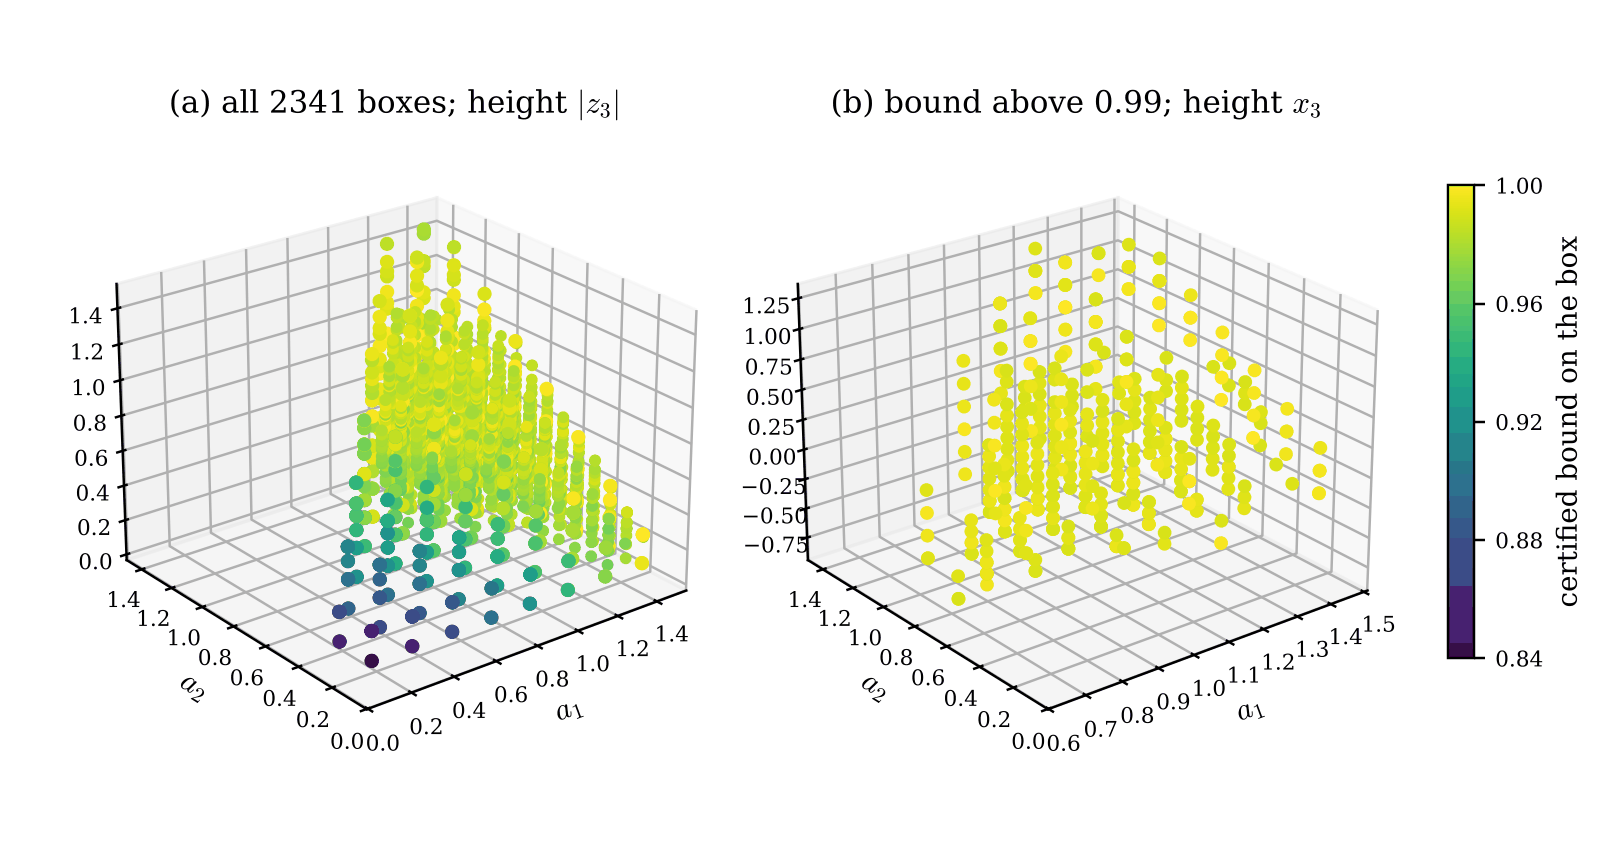
\includegraphics[width=\textwidth]{figures/fig_cover.png}
\caption{The $2341$ certified boxes at $r=\frac32$, plotted at their
centres in the coordinates $(a_1,a_2)$ of the staple sum
$\operatorname{diag}(a_1,a_2,x_3+iy_3)$, coloured by the certified bound on
$2r\sup_hL_h$ over the box; the larger points are the boxes of side $r/8$.
(a) All boxes, with height $|x_3+iy_3|$. (b) The $419$ boxes with bound
above $0.99$, with height $x_3$; the largest bounds sit in the interior of
$\mathcal R_r$, not at its extreme points.}
\label{fig:cover}
\end{figure}

\section{SU(3) with plaquette blocks}\label{sec:su3blocks}

In this section $G=\SU(3)$, $\beta\ge0$, $\beta_W=9\beta$, $N\beta=\beta_W/3$,
and the notation is that of Section~\ref{sec:su3}: $d$ is the Hilbert--Schmidt
distance, $K=\operatorname{conv}\SU(3)$, $\nu_c(dU)\propto e^{\ReTr(Uc)}dU$,
$\varphi_h(U)=\ReTr(Uh)$ and $\Lambda(r)$ is the modulus
of~\eqref{eq:alpha}. Put $Z(c)=\int e^{\ReTr(Uc)}dU$ and $g=\log Z$ on
$\C^{3\times3}$, viewed as $\R^{18}$ with the inner product $\ip
xy=\ReTr(xy^*)$. The gradient of $g$ at $c$ is the conjugate mean
$m(c)^*$, $m(c)=\nu_c(U)\in K$, and $\Hess g(c)(h,h)=\Var_{\nu_c}(\varphi_h)$.
Since $Z(VcW)=Z(c)$ for $V,W\in\SU(3)$, the same holds for $g$.

The blocks are those of Lemma~\ref{lem:plaqblocks}, which concerns the line
field only and holds for every group. For a block plaquette with active
links $e_1,e_2,e_3$, $\ReTr Q_p=\ReTr(y_1y_2y_3)$ with $y_i=Q_{e_i}$ or
$Q_{e_i}^{-1}$, and the conditional law of the block is
\begin{equation}\label{eq:blocklaw3}
\mu_b(dy)\propto\exp\Bigl(\sum_i\ReTr(y_ib_i)+N\beta\ReTr(y_1y_2y_3)
\Bigr)dy ,
\end{equation}
where $b_i$ is $N\beta$ times the sum of the five staples of $y_i$ outside
the block plaquette, so $b_i\in5N\beta K$ and $\|b_i\|_{\rm op}\le5N\beta$.
On $\SU(3)^3$ we use $d(y,y')=\sum_i\|y_i-y'_i\|_{\rm HS}$.

\subsection{The sensitivity of one block}

Let $r=2\beta_W=6N\beta$. Let $\lambda_*$ and $\tau$ be a lower and an upper
bound for the eigenvalues of $\Hess g$ on $rK$, $M$ an upper bound on $rK$
for $|D^3g(c)(u,v,v)|$ over unit vectors $u,v$, and $\gamma=\gamma(r)$ the
gap of Lemma~\ref{lem:gap}. Put
\begin{equation}\label{eq:blockconst3}
\begin{gathered}
w=\tfrac32(N\beta)^2(\tau-\lambda_*),\qquad s=\Lambda(r)+(e^w-1)e^w
\sqrt{\tau/\gamma},\\
C=5(N\beta)^2\Bigl(\tau s+\frac{\sqrt3\,N\beta\,M\,e^w}{\gamma}\Bigr),\\
K_3=\frac{(1+N\beta\Lambda(r))\,s}{1-C},\qquad\alpha_3=10N\beta K_3,
\end{gathered}
\end{equation}
assuming $C<1$.

\begin{lemma}\label{lem:onesite3}
Let $a,c_0\in5N\beta K$ and
\[
\kappa(dx)\propto\exp\bigl(\ReTr(xa)+g(c_0+N\beta x)\bigr)dx\quad\text{on }
\SU(3).
\]
For every $1$-Lipschitz $f$ and every $h\in\C^{3\times3}$:
\begin{enumerate}[label=\textup{(\roman*)},leftmargin=*]
\item $\Cov_\kappa(f,\varphi_h)\le s\|h\|_{\rm HS}$;
\item if $c_0$ moves in the direction $k$ inside $5N\beta K$, then
\[
\bigl|\tfrac{d}{dt}\kappa(f)\bigr|\le N\beta\bigl(\tau s+\sqrt3N\beta
Me^w/\gamma\bigr)\|k\|_{\rm HS}.
\]
\end{enumerate}
\end{lemma}

\begin{proof}
(i) The segment from $c_0$ to $c_0+N\beta x$ lies in $6N\beta K=rK$, and
Taylor's formula gives
\[
g(c_0+N\beta x)=g(c_0)+N\beta\ReTr(x\,m(c_0))+R(x)
\]
with $R(x)=\frac12(N\beta)^2\Hess g(\xi)(x,x)$. Since $\|x\|_{\rm HS}^2=3$,
$R\in[\frac32(N\beta)^2\lambda_*,\frac32(N\beta)^2\tau]$ and $\operatorname{osc}
R\le w$. Hence $\kappa$ is the tilt $e^R\nu/\nu(e^R)$ of $\nu=\nu_{c'}$ with
$c'=a+N\beta m(c_0)\in rK$. By definition of $\Lambda$, $\Cov_\nu(f,\varphi_h)
\le\Lambda(r)\|h\|$. The function $f$ is $1$-Lipschitz for the geodesic
distance, which dominates $d$, so $\mathrm{sd}_\nu f\le\gamma^{-1/2}$ by
Lemma~\ref{lem:gap}, and $\mathrm{sd}_\nu\varphi_h\le\sqrt\tau\|h\|$.
Lemma~\ref{lem:tilt} gives (i).

(ii) The derivative is $\Cov_\kappa(f,\ip{\nabla g(c_0+N\beta x)}k)$. Write
$\nabla g(c_0+N\beta u)=\nabla g(c_0)+N\beta\Hess g(c_0)u+N(u)$. The linear
term is $\varphi_h$ with $\|h\|\le N\beta\tau\|k\|$ and contributes at most
$N\beta\tau s\|k\|$ by (i). On the segment from $c_0$ the Hessian moves by at
most $N\beta M\|u\|\le\sqrt3N\beta M$, so $x\mapsto\ip{N(x)}k$ is
$\sqrt3(N\beta)^2M\|k\|$-Lipschitz for $d$. The law $\kappa$ is a tilt of
$\nu$ by a function of oscillation at most $w$, so its spectral gap is at
least $e^{-w}\gamma$ by the Holley--Stroock lemma~\cite{HS87}, and the
covariance of two Lipschitz functions under $\kappa$ is at most $e^w/\gamma$
times the product of their constants.
\end{proof}

\begin{lemma}\label{lem:blockK3}
Let $C<1$. If $b,b'$ have all fields in $5N\beta K$ and differ only in $b_i$,
then $W_1(\mu_b,\mu_{b'})\le K_3\|b_i-b'_i\|_{\rm HS}$ for the metric $d$.
\end{lemma}

\begin{proof}
By the cyclic symmetry of $\ReTr(y_1y_2y_3)$ we may take $i=1$. Given
$y_1,y_3$, the law of $y_2$ is $\nu_c$ with $c=b_2+N\beta y_3y_1\in rK$.
Changing $y_1$ by $\eta$ in $d$ moves $c$ by $N\beta\eta$ and $\nu_c$ by at most
$N\beta\Lambda(r)\eta$ in $W_1$, as in~\eqref{eq:alpha}; so $F(y_1,y_3)=
\E[f\mid y_1,y_3]$ is $(1+N\beta\Lambda(r))$-Lipschitz in each variable. The
law of $(y_1,y_3)$ is proportional to $e^{\ReTr(y_1b_1)+\ReTr(y_3b_3)}
Z(b_2+N\beta y_3y_1)$, and $Z(b_2+N\beta y_3y_1)=Z(y_3^{-1}b_2+N\beta y_1)=
Z(b_2y_1^{-1}+N\beta y_3)$, so its two conditional laws have the form of
Lemma~\ref{lem:onesite3}, with $c_0=y_3^{-1}b_2$ and $c_0=b_2y_1^{-1}$.
Moving $y_3$ to $y'_3$ moves $y_3^{-1}b_2$ along a segment in $5N\beta K$ of
length at most $\|b_2\|_{\rm op}\|y_3-y'_3\|\le5N\beta\|y_3-y'_3\|$. The
coupling argument of Lemma~\ref{lem:blockK} now gives $d_1\le s\varepsilon+
Cd_3$, $d_3\le Cd_1$ and $|\mu_b(f)-\mu_{b'}(f)|\le(1+N\beta\Lambda(r))(d_1+
d_3)\le K_3\varepsilon$.
\end{proof}

\subsection{The constants and the proof of Theorem~\ref{thm:su3blocks}}

\begin{lemma}\label{lem:su3const}
At $r=\frac32$ every eigenvalue of $\Hess g$ on $rK$ lies in
$[0.056015,0.247316]$, and $|D^3g(c)(u,v,v)|\le0.182126$ for $c\in rK$ and
unit vectors $u,v$. At $r=\frac{38}{25}$ the same holds with
$[0.054978,0.248280]$ and $0.183546$.
\end{lemma}

\begin{proof}
For $V,W\in\SU(3)$, $g(VcW)=g(c)$ and $x\mapsto VxW$ is an isometry, so the
eigenvalues of $\Hess g$ and the norm of $D^3g$ are constant on the orbits,
and by Lemma~\ref{lem:orbits} it suffices to bound them on $\mathcal R_r$. The
derivatives of $g$ are the cumulants of $\varphi$ under $\nu_c$. Cut the box
$[0,r]^2\times[-r,r]\times[0,r]$ into boxes of side $r/8$ and keep the $841$
($784$ at $r=\frac{38}{25}$) that survive the two tests of Section~\ref{ssec:cover}. On each box $Q$ we
compute, with rigorous error bounds, the moments of $\varphi$ of degree at
most three at the sixteen corners $b_i$ and at the centre $b_0$, and put
$k=m(b_0)$, the mean of $\varphi$ at the centre.

\emph{Upper bound.} For $b\in Q$ and every $h$, $\Var_{\nu_b}(\varphi_h)\le
\nu_b[(\varphi_h-\ip kh)^2]\le e^{\varsigma/8}\max_i\nu_{b_i}[(\varphi_h-
\ip kh)^2]$ by Lemma~\ref{lem:boxes}(ii).

\emph{Lower bound.} Integrating the right inequality of~\eqref{eq:hoeffding}
against $f\ge0$ and dividing by $Z(b)\le\sum_i\omega_iZ(b_i)$, the left one,
gives $\nu_b(f)\ge
e^{-\varsigma/8}\min_i\nu_{b_i}(f)$. With $f=(\varphi_h-\nu_b\varphi_h)^2$ this
gives $\Var_{\nu_b}(\varphi_h)\ge e^{-\varsigma/8}\min_i\Var_{\nu_{b_i}}
(\varphi_h)$.

\emph{Third cumulant.} Put $\delta=m(b)-k$. The mean value theorem and the
upper bound give $\|\delta\|\le\tau\rho+e$, with $\rho$ the largest distance
from $b_0$ in $Q$ and $e$ the error of the computed mean. Expanding the
central moment about $k$,
\[
\begin{aligned}
D^3g(b)(u,v,v)&=T_b(u,v,v)-\delta_u\Var(\varphi_v)\\
&\quad-2\delta_v\Cov(\varphi_u,\varphi_v)-\delta_u\delta_v^2 ,
\end{aligned}
\]
with $T_b=\nu_b[(\varphi-k)^{\otimes3}]$, $\delta_u=\ip\delta u$ and the
moments under $\nu_b$. For a function $G$ of either sign, writing $G=G^+-G^-$
and applying the two bounds above to $G^\pm$ gives
$|\nu_b(G)|\le(\max_i|\nu_{b_i}(G)|+\varepsilon\max_i\nu_{b_i}|G|)/(1-
\varepsilon)$ with $\varepsilon=1-e^{-\varsigma/8}$. For $G=(\varphi_u-k_u)
(\varphi_v-k_v)^2$ we use $|\nu_{b_i}(G)|\le\|T_{b_i}\|$, the largest singular
value of the $18\times324$ unfolding of $T_{b_i}$, and $\nu_{b_i}|G|\le2\sqrt3
\,\nu_{b_i}[(\varphi_v-k_v)^2]$, since $\|U-k\|_{\rm HS}\le2\sqrt3$. The
largest eigenvalues and singular values are bounded as in
Section~\ref{ssec:cover}, and the maxima over these boxes are the numbers
stated (Appendix~\ref{app:plaqblocks}).
\end{proof}

\begin{proof}[Proof of Theorem~\ref{thm:su3blocks}]
Let first $\beta_W\le\frac34$, so that $r=2\beta_W\le\frac32$. Every field
met in Lemmas~\ref{lem:onesite3} and~\ref{lem:blockK3} lies in $\frac32K$, so
the constants of Lemma~\ref{lem:su3const} at $\frac32$,
$\Lambda(\frac32)\le\frac{0.999887}3$ from Proposition~\ref{prop:cover} and
$\gamma=\gamma(\frac32)=\frac{187}{128}$ apply; with these fixed constants every
quantity in~\eqref{eq:blockconst3} is increasing in $\beta_W$. For
$\frac34<\beta_W\le\frac{19}{25}$ the fields lie in $\frac{38}{25}K$, and the
constants of Lemma~\ref{lem:su3const} at $\frac{38}{25}$,
$\Lambda(\frac{38}{25})\le\frac{1.029967}{3.04}$ from
Proposition~\ref{prop:cover2} and $\gamma(\frac{38}{25})=\frac{4643}{3200}$
apply in the same way. Changing an active link $j$ by $\eta$ changes one
staple of each of its ten partners outside its block by a matrix of norm
$\eta$, so the field $b_i$ of each such partner moves by $N\beta\eta$, and
Lemma~\ref{lem:blockK3} gives $\sum_BC_{Bj}\le10N\beta K_3=\alpha_3(\beta_W)$.
In ball arithmetic, at $\beta_W=\frac34$, $w\le0.017935$, $s\le0.34088$,
$C\le0.043520$, $K_3\le0.38609$ and $\alpha_3\le0.96521$; at $\beta_W=0.72$,
$\alpha_3\le0.91815$; at $\beta_W=0.76$, with the second set of constants,
$w\le0.018609$, $s\le0.34673$, $C\le0.045770$, $K_3\le0.39454$ and
$\alpha_3\le0.99950$. Proposition~\ref{prop:blockstate}, whose proof does not
use the group, applies with the Hilbert--Schmidt metric.
\end{proof}

\begin{remark}\label{rem:su3blocks}
Theorem~\ref{thm:su3} ends where $2r\Lambda(r)$ reaches one. The blocks
remove the factor $\frac{12}{10}$ of the single-link sum and keep most of it
after paying for the three links: at $\beta_W=\frac34$ the gap bound rises
from $1.1\cdot10^{-4}$ to $0.0177$, and the block bound is the better one for
$\beta_W\ge0.715$. Before the corrections for the three links their sum is
$\frac{10}{12}$ of the single-link sum $2r\Lambda(r)$, so it can stay below one
while $2r\Lambda(r)$ is slightly above one; Proposition~\ref{prop:cover2} certifies
$2r\Lambda(r)\le1.03$ at $r=1.52$, which is enough at $\beta_W=0.76$, with
little room. Evaluated in floating point with the constants of a scan of
$\mathcal R_r$, the block sum stays below one up to $\beta_W\approx0.78$;
that computation is not certified and is not used.
\end{remark}

\section{Where the methods stop}\label{sec:limits}

\emph{$\SU(2)$.} Theorem~\ref{thm:ceiling} closes the single-link route in
every forest gauge at $\beta_W=\frac13$. Blocks of several links, where the
influence of a boundary link on a whole block is bounded at once, in the
spirit of the Dobrushin--Shlosman criterion~\cite{DS85}, pass it:
plaquette blocks reach $\beta_W=0.345$ (Theorem~\ref{thm:blocks}), and the
sharper floating-point bound of Remark~\ref{rem:blockgap} stops near
$0.357$. Larger blocks are the next step.

\emph{Curvature.} Remark~\ref{rem:hf} locates the end of the curvature
method in this gauge between $|\beta|=\frac1{29}$ and $\frac1{26.25}$.

\emph{$\SU(3)$.} The route of Section~\ref{sec:su3} bounds the
$H^{-1}(\nu_b)$ norm of $\varphi_h-\nu_b\varphi_h$, which is at least
$L_h(b)$, and needs it uniformly on $rK$. Its Galerkin values (polynomials
of degree two) at matrices of $rK$ give $2r$ times the norm equal to $0.79$
at $r=1.25$, $0.89$ at $r=1.4$, $0.97$ at $r=1.5$ and $1.009$ at $r=1.55$, so
the route stops at or below $\beta_W\approx0.77$ even with exact constants.
With $u=s\varphi_h$, Lemma~\ref{lem:corrector} stops earlier: in floating
point its largest values on $\mathcal R_r$ lie on the face
$\operatorname{diag}(r,\rho,\rho)$ with $\rho$ between $0.75r$ and $0.8r$, and
$2r$ times the bound is $0.9458$ at $r=1.36$, $0.9767$ at $r=1.40$ and $1.0080$
at $r=1.44$, so this corrector ends near $\beta_W\approx0.715$. With $u=q_h$
of degree two the largest values on the same face are $0.9305$ at $r=1.44$,
$0.9729$ at $r=1.50$ and $1.0018$ at $r=1.54$ (Figure~\ref{fig:face}), close to the
Galerkin values. Lemma~\ref{lem:gap} therefore costs
little at these couplings, and most of the distance between the
floating-point value at $r=1.5$ and the certified $0.999887$ of
Proposition~\ref{prop:cover} is the interpolation over boxes. Between
$\beta_W=\frac34$ and $0.77$ there is room only for smaller boxes. The
plaquette blocks of Theorem~\ref{thm:su3blocks} use $\Lambda(2\beta_W)$ as
well, with a little more room: they reach $0.76$ with the certified cover of
Proposition~\ref{prop:cover2} and near $0.78$ in floating point
(Remark~\ref{rem:su3blocks}); past that one needs larger blocks, whose
sensitivity does not go through the one-link modulus.

\begin{figure}[tb]
\centering
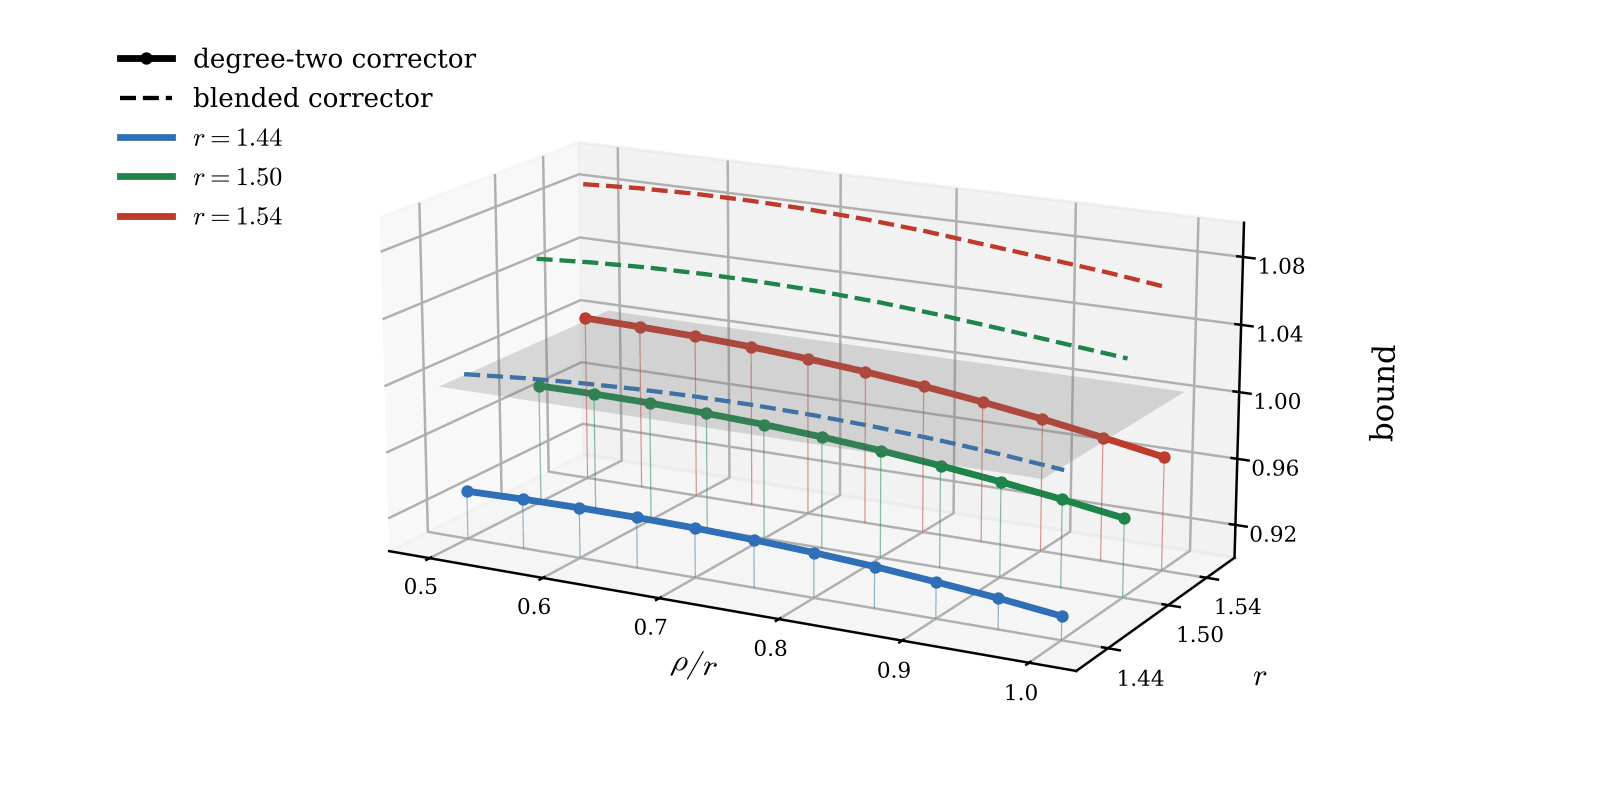
\includegraphics[width=\textwidth]{figures/fig_face.png}
\caption{The floating-point value of $2r\sup_h$ of the bound of
Lemma~\ref{lem:corrector} on the face $b=\operatorname{diag}(r,\rho,\rho)$, as
a function of $\rho/r$, for $r=1.44$, $1.50$ and $1.54$: dashed with the
corrector $u=s\varphi_h$ for the best $s$, solid with $u=q_h$ of degree two
for the best $C$. The grey plane is the Dobrushin threshold one. The first
corrector is above it already at $r=1.44$; the second stays below it at
$r=1.50$, where Proposition~\ref{prop:cover} certifies the bound on all of
$\mathcal R_r$, and crosses it by $r=1.54$.}
\label{fig:face}
\end{figure}

\emph{The four open problems.} Our earlier paper~\cite{BB26a} listed four
problems between the strong-coupling results and the Clay
problem~\cite{JW06}: (1) uniqueness and a gap at intermediate fixed
coupling; (2) the crossover from strong coupling to Ba{\l}aban's
weak-coupling regime; (3) the continuum limit with the
Osterwalder--Schrader axioms; and (4) a gap in physical units. The present
paper moves the boundary of (1): for $\SU(2)$ from $\beta_W=\frac29$ to
$0.345$, for $\SU(3)$ from $\frac9{32}$ to $0.76$, with a gap at $\frac34$ of
$0.0177$ in lattice units, and for every
$\SU(N)$ past the curvature ceiling. It does not close (1); the region
between these values and the scaling region, near $\beta_W\approx2.2$ for
$\SU(2)$ and $\beta_W\approx6$ for $\SU(3)$, is open, and with it problem
(2). Problems (3) and (4) are untouched. Every bound proved here is uniform
in lattice units, so by~\cite{BB26b} none of them can by itself produce a
continuum mass gap; that requires control of the gap in physical units along
the renormalisation group flow~\cite{Bal84a,BSB26}.

\section*{Declarations}

\subsection*{Data availability}
The analytic proofs are complete as written, except the evaluations in
Propositions~\ref{prop:cover} and~\ref{prop:cover2} and
Lemma~\ref{lem:su3const} and the numerical bounds of
Lemma~\ref{lem:vmfconst}, which are computations with rigorous error bounds,
and the finite check of Lemma~\ref{lem:plaqblocks}. The archive
\texttt{creelie/4Y-M} (release v3.4.0,
\url{https://github.com/creelie/4y-m/releases/tag/v3.4.0}; all versions on
Zenodo,
\href{https://doi.org/10.5281/zenodo.23444338}{doi:10.5281/zenodo.23444338})
contains the programs of that computation, in Python with python-flint
(FLINT and Arb) and a C kernel for products of Taylor polynomials, with
their outputs and the list of certified boxes; the programs and outputs of
the earlier certificate at $\beta_W=\frac{45}{64}$;
independent checks in exact rational arithmetic of Lemmas~\ref{lem:local}
and~\ref{lem:roughlap} and of~\eqref{eq:pointwise}; numerical checks of
Lemma~\ref{lem:identity} on tori; the searches of Remark~\ref{rem:hf} and
Section~\ref{sec:limits}; a Lean~4 certificate of the line field
(Lemmas~\ref{lem:cycle} and~\ref{lem:structure} for the table of
Appendix~\ref{app:table}, by \texttt{decide}); the programs of
Appendix~\ref{app:plaqblocks} for the plaquette blocks, with the
floating-point search of Remark~\ref{rem:blockgap}; and the source of the
preprint version of this paper. Deep Bhattacharjee carried out the
computations and the Lean, Python and shell checks with AI assistance from
Claude (Anthropic). The first composite behind Theorem~\ref{thm:su2} was
assembled by Anaxia, the reasoning engine of the BLLM system, in release
v3.0.5~\cite{Bha26}, as described in the footnote to that theorem; release
v3.1.0~\cite{Bha26b} records the engine's Yang--Mills runs in its failure
log, whose last Yang--Mills entry is the change from single links to blocks
of several links; the plaquette blocks of Section~\ref{sec:plaqblocks}, the bound of Lemma~\ref{lem:blockK}, their $\SU(3)$ version in
Section~\ref{sec:su3blocks} and the certified constants were found and
checked by the authors. Both authors approved the final text.

\subsection*{Funding}
None.

\subsection*{Competing interests}
None.


\appendix

\section{The line field}\label{app:table}

Table~\ref{tab:sigma} lists, for each residue class of $x$ modulo two, the
direction $\sigma(x)$ and the permutation $\pi_x(\mu)=\sigma(x+e_\mu)$. In every
row $\pi_x$ fixes $\sigma(x)$ and is a three-cycle on the other directions,
which is the condition of Lemma~\ref{lem:cycle}.

\begin{table}[h]
\caption{The line field: $x$ modulo two (digits $x_0x_1x_2x_3$), the
direction $\sigma(x)$ and the values $\sigma(x+e_\mu)$ for $\mu=0,1,2,3$.}
\label{tab:sigma}
\begin{tabular}{cccccc}
\toprule
$x$&$\sigma(x)$&$\mu=0$&$\mu=1$&$\mu=2$&$\mu=3$\\
\midrule
0000 & 0 & 0 & 2 & 3 & 1 \\
1000 & 0 & 0 & 3 & 1 & 2 \\
0100 & 2 & 3 & 0 & 2 & 1 \\
1100 & 3 & 2 & 0 & 1 & 3 \\
0010 & 3 & 1 & 2 & 0 & 3 \\
1010 & 1 & 3 & 1 & 0 & 2 \\
0110 & 2 & 1 & 3 & 2 & 0 \\
1110 & 1 & 2 & 1 & 3 & 0 \\
0001 & 1 & 2 & 1 & 3 & 0 \\
1001 & 2 & 1 & 3 & 2 & 0 \\
0101 & 1 & 3 & 1 & 0 & 2 \\
1101 & 3 & 1 & 2 & 0 & 3 \\
0011 & 3 & 2 & 0 & 1 & 3 \\
1011 & 2 & 3 & 0 & 2 & 1 \\
0111 & 0 & 0 & 3 & 1 & 2 \\
1111 & 0 & 0 & 2 & 3 & 1 \\
\bottomrule
\end{tabular}
\end{table}

\section{The comparison lemma}\label{app:comparison}

Let $(G,\delta)$ be a compact group with a bi-invariant metric of diameter
$D$, $\Omega=G^A$, and $C_{ee'}$ the coefficients of Section~\ref{sec:state},
with row and column sums at most $\alpha<1$ and $C_{ee'}=0$ unless $e,e'$ share
a plaquette, so that $|e-e'|\le1$ for the distance of link midpoints. Fix
$\lambda>0$ with $\theta=\alpha e^\lambda<1$.

\begin{lemma}\label{lem:comparison}
Let $S\subset A$, possibly infinite, and let $\mu_1,\mu_2$ be probability
measures on $\Omega$ invariant under $\gamma^F_e$ for every $e\notin S$. Let
$T\subset A\setminus S$ be finite, $w_b=e^{-\lambda\dist(b,T)}$, and suppose
$\sum_{z\in S}w_z<\infty$. There is a coupling of $\mu_1,\mu_2$ whose link
distances $\varrho(b)=\E\,\delta(\sigma_b,\sigma'_b)$ satisfy
\[
\sum_{b\notin S}w_b\varrho(b)\le\frac{\theta D}{1-\theta}\sum_{z\in S}w_z .
\]
If $S=\emptyset$ then $\mu_1=\mu_2$.
\end{lemma}

\begin{proof}
The couplings form a weakly compact set and $\Psi(\pi)=\sum_bw_b\E_\pi\delta(
\sigma_b,\sigma'_b)$ is weakly continuous because $\sum_bw_b<\infty$; let $\pi^*$ be
a minimiser. For $e\notin S$ replace the pair $(\sigma_e,\sigma'_e)$ by a sample of
an optimal coupling of $\gamma^F_e(\cdot\mid\sigma)$ and $\gamma^F_e(\cdot\mid
\sigma')$, chosen measurably~\cite[Cor.~5.22]{Vil09}. Both $\mu_i$ are
invariant, so the result is again a coupling, and changing the finitely
many links that enter $\gamma^F_e$ one at a time gives $W_1\le\sum_{e'}C_{ee'}
\delta(\sigma_{e'},\sigma'_{e'})$. Minimality gives $\varrho(e)\le\sum_{e'}C_{ee'}
\varrho(e')$. Multiply by $w_e$ and sum over $e\notin S$; where $C_{ee'}\ne0$,
$w_e\le e^\lambda w_{e'}$, so
\[
\sum_{e\notin S}w_e\varrho(e)\le\theta\Bigl[\sum_{e'\notin S}w_{e'}\varrho(e')
+\sum_{z\in S}w_z\varrho(z)\Bigr],
\]
all sums are finite, and $\varrho\le D$ on $S$. If $S=\emptyset$, $\varrho\equiv0$.
\end{proof}

\begin{corollary}\label{cor:decay}
Let $\mu$ be the Gibbs measure of $\gamma^F$, $F$ a local function with
support $S_F$, $L_F$-Lipschitz in each link, and $H$ bounded with finite
support $S_H$ disjoint from $S_F$. Then
\[
|\Cov_\mu(F,H)|\le\|H\|_\infty L_F\frac{\theta D}{1-\theta}|S_H|\,
e^{-\lambda\dist(S_F,S_H)}.
\]
\end{corollary}

\begin{proof}
Condition on the links of $S_H$~\cite[Ch.~3]{Kal21}; the conditional
measures are invariant under $\gamma^F_e$ for $e\notin S_H$, and
Lemma~\ref{lem:comparison} with $S=S_H$, $T=S_F$ bounds the difference of
two of them, as in~\cite[Cor.~29]{BB26a}.
\end{proof}

\begin{lemma}\label{lem:blockcomparison}
Let the blocks partition $A$, let $C_{Bj}$ be the block coefficients of
Section~\ref{sec:plaqblocks}, with $\sum_BC_{Bj}\le\alpha<1$ for every $j$ and
$C_{Bj}=0$ unless every link of $B$ lies within distance $2$ of $j$, and fix
$\lambda>0$ with $\theta=\alpha e^{2\lambda}<1$. Let $S\subset A$ be a union
of blocks and let $\mu_1,\mu_2$ be invariant under $\gamma^{\mathcal B}_B$ for
every block $B\not\subset S$. With $T$, $w_b$ as in
Lemma~\ref{lem:comparison} and $\sum_{z\in S}w_z<\infty$, there is a coupling
with $\sum_{b\notin S}w_b\varrho(b)\le\frac{\theta D}{1-\theta}\sum_{z\in S}w_z$,
and $\mu_1=\mu_2$ if $S=\emptyset$.
\end{lemma}

\begin{proof}
Take a minimiser $\pi^*$ of $\Psi$ as before. For a block $B\not\subset S$
replace $(\sigma_B,\sigma'_B)$ by an optimal coupling, for the metric $d$, of
the two block laws; it is again a coupling, and changing the boundary links
one at a time bounds the expected new $d$-distance by $\sum_jC_{Bj}\varrho(j)$.
Put $\bar w_B=\max_{i\in B}w_i$. Minimality gives
\[
\sum_{i\in B}w_i\varrho(i)\le\bar w_B\sum_jC_{Bj}\varrho(j),
\]
and $\bar w_B\le e^{2\lambda}w_j$ whenever $C_{Bj}\ne0$. Summing over the
blocks outside $S$ and using the column sums,
\[
\sum_{b\notin S}w_b\varrho(b)\le\theta\Bigl[\sum_{j\notin S}w_j\varrho(j)+
\sum_{z\in S}w_z\varrho(z)\Bigr],
\]
which gives the claim as in Lemma~\ref{lem:comparison}.
\end{proof}

\section{The plaquette blocks}\label{app:plaqblocks}

Table~\ref{tab:plaqblocks} lists the block plaquettes of
Section~\ref{sec:plaqblocks} modulo $2\Z^4$: the plaquette at $x$ in the plane
$\{\mu,\nu\}$ is a block plaquette exactly when $x$ modulo two and
$\{\mu,\nu\}$ appear in the table. Eight lie in the plane $\{0,1\}$ and eight
in $\{2,3\}$; together they contain the $48$ active links of a cell of side
two, each once.

\begin{table}[h]
\caption{The sixteen block plaquettes modulo two: the base point $x$
(digits $x_0x_1x_2x_3$ modulo two) and the plane.}
\label{tab:plaqblocks}
\centering
\begin{tabular}{cccc}
\toprule
$x$&plane&$x$&plane\\
\midrule
0000&$\{0,1\}$&0000&$\{2,3\}$\\
0001&$\{0,1\}$&0011&$\{2,3\}$\\
0010&$\{0,1\}$&0100&$\{2,3\}$\\
0011&$\{0,1\}$&0111&$\{2,3\}$\\
1100&$\{0,1\}$&1000&$\{2,3\}$\\
1101&$\{0,1\}$&1011&$\{2,3\}$\\
1110&$\{0,1\}$&1100&$\{2,3\}$\\
1111&$\{0,1\}$&1111&$\{2,3\}$\\
\bottomrule
\end{tabular}
\end{table}

The program \texttt{cover.py} in the folder
\nolinkurl{strong-coupling/gauge-fixed/blocks/} of the archive finds this set by an exact-cover search on the torus of side
two and checks Lemma~\ref{lem:plaqblocks} on the tori of side four and six.
The program \texttt{constants.py} evaluates the bounds of
Lemma~\ref{lem:vmfconst} in ball arithmetic with python-flint at $120$ bits:
the series of $Z_0$ and of its first three derivatives in $s=r^2$ is summed to
forty terms, and the tail is bounded for $s\le5$ by twice the first omitted
term $(5/4)^{40}40^3/(40!\,41!)$, because consecutive terms decrease by a
factor below one half. The program \texttt{alpha.py} evaluates the constants
of~\eqref{eq:blockconst} and $\alpha$ at a given $\beta_W$, read exactly.

For $\SU(3)$ the folder \nolinkurl{strong-coupling/gauge-fixed/blocks/su3/}
contains \texttt{consts.py}, which evaluates the bounds of
Lemma~\ref{lem:su3const} on the $841$ boxes of side $\frac3{16}$ at
$r=\frac32$ and the $784$ boxes of side $\frac{19}{100}$ at $r=\frac{38}{25}$
with the moments of Appendix~\ref{app:cover}, and \texttt{alpha3.py}, which
reads these bounds and the cover of Proposition~\ref{prop:cover} or
Proposition~\ref{prop:cover2} and evaluates the constants
of~\eqref{eq:blockconst3} and $\alpha_3$ in ball arithmetic at $120$ bits; its
outputs at $\beta_W=\frac34$ and $0.76$ are listed with the bounds of each box.
The cover of Proposition~\ref{prop:cover2} is computed by the program of
Appendix~\ref{app:cover} with \texttt{--r 38/25 --thr 1.03}.

\section{The blocks of Lemma~\ref{lem:local}}\label{app:blocks}

\emph{Diagonal blocks.} Let $w_a=e^{i\phi}$. On the diagonal part,
$f_p=-\cos\phi\,(y_1+y_2-y_3-y_4)^2$ and $c_p=2(y_1y_4-y_1y_2+y_2y_3-y_3y_4)$, so
\[
\begin{split}
\mathcal F={}&\sum_i\alpha_iy_i^2+\cos\phi\,(y_1+y_2-y_3-y_4)^2\\
&-\tfrac95(y_1y_4-y_1y_2+y_2y_3-y_3y_4)
\end{split}
\]
with $y_k=0$ and weights $\alpha_{k\pm1}=\frac{21}{10}$, $\alpha_{k+2}=\frac54$.
It is affine in $\cos\phi$, so positivity at $\cos\phi=\pm1$ suffices. For
$k=1$ and $\cos\phi=1$ the matrix in $(y_2,y_3,y_4)$ is
\[
\begin{pmatrix}\frac{31}{10}&-\frac{19}{10}&-1\\[2pt]-\frac{19}{10}&\frac94&
\frac{19}{10}\\[2pt]-1&\frac{19}{10}&\frac{31}{10}\end{pmatrix},
\]
and Table~\ref{tab:minors} lists the leading principal minors for every
position; all are positive.

\begin{table}[h]
\caption{Leading principal minors of the diagonal blocks of
Lemma~\ref{lem:local}.}
\label{tab:minors}
\begin{tabular}{lll}
\toprule
Fixed link&$\cos\phi=1$&$\cos\phi=-1$\\
\midrule
$e_1$, $e_4$&$\frac{31}{10},\ \frac{673}{200},\ \frac{8421}{2000}$&
$\frac{11}{10},\ \frac{53}{200},\ \frac{21}{2000}$\\[2pt]
$e_2$&$\frac{31}{10},\ \frac{861}{100},\ \frac{8421}{2000}$&
$\frac{11}{10},\ \frac{21}{100},\ \frac{21}{2000}$\\[2pt]
$e_3$&$\frac94,\ \frac{673}{200},\ \frac{8421}{2000}$&
$\frac14,\ \frac{53}{200},\ \frac{21}{2000}$\\
\bottomrule
\end{tabular}
\end{table}

\emph{Pair blocks.} Let $w_a=e^{i(\chi+\vartheta)}$ and $w_b=e^{i(\chi-\vartheta)}$.
The terms of $f_p$ carry $w_a+\bar w_b=2\cos\chi\,e^{i\vartheta}$ or its
conjugate, and $c_p$ carries $w_a\bar w_b=e^{2i\vartheta}$, so the Hermitian
matrix $M(m,\vartheta)$ of $\mathcal F$, $m=\cos\chi$, is affine in $m$ with
$M(-1,\vartheta)=M(1,\vartheta+\pi)$, and $m=1$ suffices. For the fixed link
$e_2$, in the variables $(z_1,z_3,z_4)$ and with $c=\cos\vartheta$,
\[
M=\begin{pmatrix}\frac{21}5+2c&-2e^{i\vartheta}&-\frac95-2e^{i\vartheta}\\[2pt]
-2e^{-i\vartheta}&\frac{21}5+2c&\frac95+2e^{-i\vartheta}\\[2pt]
-\frac95-2e^{-i\vartheta}&\frac95+2e^{i\vartheta}&\frac52+2c\end{pmatrix}.
\]
With $u=\cos^2(\vartheta/2)\in[0,1]$ its leading principal minors are
\[
\tfrac{20u+11}5,\quad\tfrac{(20u+1)(20u+21)}{25},\quad
\tfrac{400u(40u^2-23u+4)+21}{250},
\]
and $40u^2-23u+4$ has negative discriminant $529-640$. The other positions
give the same determinant and the leading minors $\frac{20u+11}5$ or
$\frac{8u+1}2$ and $\frac{800u^2-180u+53}{50}$, whose discriminant $32400-169600$
is negative. Every block is positive definite.

The inequality is not tight. In floating point the least eigenvalue of the
whole form over $W\in\U(N)$, $N\le4$, is $0.0149$, which is also the least
eigenvalue of the exact blocks; this slack is what the choice of the weights
$\frac{21}{10}$, $\frac54$, $\frac9{10}$ trades against the constant
$\frac{29}2$.

\section{The certified computation}\label{app:cover}

\emph{Truncation.} For a corner $b$ of a box the moments of
Lemma~\ref{lem:characters} are derivatives of $Z$ at $(b,\bar b)$. The
truncated series is $\E_H[A_t(UD)B_t(\bar UD')]$ with $A_t$ the part of
$\sum_\lambda c_\lambda s_\lambda(UD)$ over partitions with $\lambda_1-\lambda_3\le34$ and
$\lambda_3\le11$, and $B_t$ likewise. Every omitted partition has $|\lambda|>34$,
because $3\cdot12>34$, and the omitted part is at most $T(\|D\|)=\sum_{n>34}
(\frac32\|D\|)^n/n!$ in modulus. On the polydisc $|D_{ij}-b_{ij}|\le\rho$,
$\|D\|\le\|b\|+3\rho$, and Cauchy's estimate bounds the $\alpha$-th derivative
of the omitted part by $\alpha!\rho^{-|\alpha|}T(\|b\|+3\rho)$. The
derivatives of the full exponential are at most $2^{-|\alpha|}e^{v/2}$ with
$v=\sum_k|b_k|$, since $|\Tr(Ub)|\le\sum_k|b_k|$ for diagonal $b$. With
$\varepsilon_\alpha=2^{|\alpha|}\alpha!\rho^{-|\alpha|}T(\|b\|+3\rho)$ the
truncated moment differs from the true one by at most $\varepsilon_\alpha e^{v/2}
+(e^{v/2}+\varepsilon_\alpha)\varepsilon_\beta$, and $\rho$ is chosen to minimise
$\rho^{-6}T$. The largest error bound of an unnormalised moment at any corner is
$1.7\times10^{-11}$.

\emph{Weight zero.} Conjugation by the diagonal torus $T$ preserves Haar measure
and $\ReTr(Ub)$ for diagonal $b$, and multiplies $u_{ij}$ by $t_it_j^{-1}$; a
moment of a monomial on which $T$ acts by a nontrivial character is therefore
$0$, and only $8278$ of the $134596$ monomials of degree at most six have the
trivial character. The functions $\Tr(X)$, $e_2(X)$, $\det X$ of $X=DD'^\top$
and $\det D$, $\det D'$ are invariant under the same action on the variables,
so after these are formed in the full ring of Taylor polynomials of degree six
in the $18$ variables, the series is computed in the subring of weight-zero
monomials.

\emph{Rounding.} The truncated series is a Taylor polynomial of total degree
six in the $36$ real directions of $(D-b,D'-\bar b)$, computed in double
precision. Every operation is repeated on absolute values and carries an
operation count $n$, so that the computed coefficient differs from the
exact one by at most $\gamma_n=nu/(1-nu)$, $u=2^{-53}$, times the
absolute-value coefficient~\cite[Sec.~3.1]{Hig02}. With $C$ in $2^{-30}\Z$,
the polynomials $2^{31}q_h$, $X_a(2^{31}q_h)$,
$12\cdot2^{31}(\varphi_h+\Delta q_h)$ and $12\cdot2^{31}\ip{\nabla\varphi_{F_k}}
{\nabla q_h}$ for the coordinate vectors $h$ have coefficients in $\Z[i]$, and
every partial sum in their computation is bounded, through the same
operations on absolute values, by less than $2^{50}$; they are therefore
computed exactly. Normalisation by $Z$, the products with the corner
coordinates, the quadratic forms and their error matrices are formed with the
same bookkeeping, and the largest eigenvalues are bounded in ball
arithmetic~\cite{Joh17}.

\emph{Separation.} The functional $c$ of a discarded box is the dual solution
of a linear program for the gauge of the centre of the box with respect to a
$72\times72$ grid of $T$. Only the final inequality is used: $\max_T\ell$ is
bounded by its maximum over a $512\times512$ grid plus $\frac12H\delta^2/2$, with
$\delta=2\pi/512$ and $H=|c_1|+|c_2|+2|c_3|$ a bound for its Hessian on the
torus, and the inequality is checked with relative margin $10^{-12}$.

\emph{Running time.} The moments at one corner take about one and a half seconds and
the bound on one box about two and a half seconds on one core. The cover runs in about an hour on
four cores and writes every certified box with its $\theta$ and its bound.

\begin{thebibliography}{99}\raggedright

\bibitem{BE85}
Bakry, D., \'Emery, M.: Diffusions hypercontractives. In: S\'eminaire de
Probabilit\'es XIX. Lecture Notes in Math., vol.~1123, pp.~177--206.
Springer, Berlin (1985).
\href{https://doi.org/10.1007/BFb0075847}{https://doi.org/10.1007/BFb0075847}

\bibitem{BGL14}
Bakry, D., Gentil, I., Ledoux, M.: Analysis and Geometry of Markov
Diffusion Operators. Grundlehren Math. Wiss., vol.~348. Springer, Cham
(2014).
\href{https://doi.org/10.1007/978-3-319-00227-9}{https://doi.org/10.1007/978-3-319-00227-9}

\bibitem{Bal84a}
Ba{\l}aban, T.: Propagators and renormalization transformations for lattice
gauge theories.~I. Commun. Math. Phys. \textbf{95}, 17--40 (1984).
\href{https://doi.org/10.1007/BF01215753}{https://doi.org/10.1007/BF01215753}

\bibitem{Bal85a}
Ba{\l}aban, T.: Averaging operations for lattice gauge theories. Commun.
Math. Phys. \textbf{98}, 17--51 (1985).
\href{https://doi.org/10.1007/BF01211042}{https://doi.org/10.1007/BF01211042}

\bibitem{Bal89b}
Ba{\l}aban, T.: Large field renormalization. II. Localization,
exponentiation, and bounds for the $\mathbf R$ operation. Commun. Math.
Phys. \textbf{122}, 355--392 (1989).
\href{https://doi.org/10.1007/BF01238433}{https://doi.org/10.1007/BF01238433}

\bibitem{Ban38}
S.~Banach, \"Uber homogene Polynome in $(L^2)$, Studia Math. \textbf{7}
(1938), 36--44,
\href{https://doi.org/10.4064/sm-7-1-36-44}{doi:10.4064/sm-7-1-36-44}.

\bibitem{Bha26}
Bhattacharjee, D.: BLLM: Beyond the LLM with Deep Human-Mind-AI. Zenodo,
release v3.0.5 (2026).
\href{https://doi.org/10.5281/zenodo.23469389}{https://doi.org/10.5281/zenodo.23469389}

\bibitem{Bha26b}
Bhattacharjee, D.: BLLM: Beyond the LLM with Deep Human-Mind-AI. Zenodo,
release v3.1.0 (2026).
\href{https://doi.org/10.5281/zenodo.23484160}{https://doi.org/10.5281/zenodo.23484160}

\bibitem{BB26a}
Bhattacharjee, D., Bhattacharya, U.: Mass gap of lattice Yang--Mills
theory up to the Dobrushin ceiling. Zenodo, release v2.0.2 (2026).
\href{https://doi.org/10.5281/zenodo.23449466}{https://doi.org/10.5281/zenodo.23449466}

\bibitem{BB26b}
Bhattacharjee, D., Bhattacharya, U.: Spacing-uniform lattice inequalities
cannot produce the Yang--Mills mass gap. Zenodo, release v1.0.0 (2026).
\href{https://doi.org/10.5281/zenodo.23444339}{https://doi.org/10.5281/zenodo.23444339}

\bibitem{BSB26}
Bhattacharjee, D., Samal, P., Bhattacharya, S.: Geometric structure and
renormalization group flow in chiral Yang--Mills--Higgs theory. Preprints
(2026).
\href{https://doi.org/10.20944/preprints202602.2022.v1}{https://doi.org/10.20944/preprints202602.2022.v1}

\bibitem{Bum13}
Bump, D.: Lie Groups, 2nd edn. Grad. Texts in Math., vol.~225. Springer,
New York (2013).
\href{https://doi.org/10.1007/978-1-4614-8024-2}{https://doi.org/10.1007/978-1-4614-8024-2}

\bibitem{Cre77}
Creutz, M.: Gauge fixing, the transfer matrix, and confinement on a
lattice. Phys. Rev. D \textbf{15}, 1128--1136 (1977).
\href{https://doi.org/10.1103/PhysRevD.15.1128}{https://doi.org/10.1103/PhysRevD.15.1128}

\bibitem{Dob68}
Dobrushin, R.L.: The description of a random field by means of conditional
probabilities and conditions of its regularity. Theory Probab. Appl.
\textbf{13}, 197--224 (1968).
\href{https://doi.org/10.1137/1113026}{https://doi.org/10.1137/1113026}

\bibitem{Dob70}
Dobrushin, R.L.: Prescribing a system of random variables by conditional
distributions. Theory Probab. Appl. \textbf{15}, 458--486 (1970).
\href{https://doi.org/10.1137/1115049}{https://doi.org/10.1137/1115049}

\bibitem{DS85}
Dobrushin, R.L., Shlosman, S.B.: Constructive criterion for the uniqueness
of Gibbs field. In: Statistical Physics and Dynamical Systems,
pp.~347--370. Birkh\"auser, Boston (1985).
\href{https://doi.org/10.1007/978-1-4899-6653-7_20}{https://doi.org/10.1007/978-1-4899-6653-7\_20}

\bibitem{FH91}
Fulton, W., Harris, J.: Representation Theory: A First Course. Grad. Texts
in Math., vol.~129. Springer, New York (1991).
\href{https://doi.org/10.1007/978-1-4612-0979-9}{https://doi.org/10.1007/978-1-4612-0979-9}

\bibitem{GL10}
Gattringer, C., Lang, C.B.: Quantum Chromodynamics on the Lattice. Lecture
Notes in Phys., vol.~788. Springer, Berlin (2010).
\href{https://doi.org/10.1007/978-3-642-01850-3}{https://doi.org/10.1007/978-3-642-01850-3}

\bibitem{Hig02}
Higham, N.J.: Accuracy and Stability of Numerical Algorithms, 2nd edn.
SIAM, Philadelphia (2002).
\href{https://doi.org/10.1137/1.9780898718027}{https://doi.org/10.1137/1.9780898718027}

\bibitem{HS87}
R.~Holley and D.~Stroock, Logarithmic Sobolev inequalities and stochastic
Ising models, J. Stat. Phys. \textbf{46} (1987), 1159--1194,
\href{https://doi.org/10.1007/BF01011161}{doi:10.1007/BF01011161}.

\bibitem{Hoe63}
Hoeffding, W.: Probability inequalities for sums of bounded random
variables. J. Amer. Statist. Assoc. \textbf{58}, 13--30 (1963).
\href{https://doi.org/10.1080/01621459.1963.10500830}{https://doi.org/10.1080/01621459.1963.10500830}

\bibitem{JW06}
Jaffe, A., Witten, E.: Quantum Yang--Mills theory. In: The Millennium
Prize Problems, pp.~129--152. Clay Mathematics Institute, Cambridge, MA,
and American Mathematical Society, Providence, RI (2006).
\url{https://www.claymath.org/wp-content/uploads/2022/06/yangmills.pdf}

\bibitem{Joh17}
Johansson, F.: Arb: efficient arbitrary-precision midpoint-radius interval
arithmetic. IEEE Trans. Comput. \textbf{66}, 1281--1292 (2017).
\href{https://doi.org/10.1109/TC.2017.2690633}{https://doi.org/10.1109/TC.2017.2690633}

\bibitem{Kal21}
Kallenberg, O.: Foundations of Modern Probability, 3rd edn. Springer, Cham
(2021).
\href{https://doi.org/10.1007/978-3-030-61871-1}{https://doi.org/10.1007/978-3-030-61871-1}

\bibitem{KS75}
Kogut, J., Susskind, L.: Hamiltonian formulation of Wilson's lattice gauge
theories. Phys. Rev. D \textbf{11}, 395--408 (1975).
\href{https://doi.org/10.1103/PhysRevD.11.395}{https://doi.org/10.1103/PhysRevD.11.395}

\bibitem{MM94}
Montvay, I., M\"unster, G.: Quantum Fields on a Lattice. Cambridge
University Press, Cambridge (1994).
\href{https://doi.org/10.1017/CBO9780511470783}{https://doi.org/10.1017/CBO9780511470783}

\bibitem{OS73}
Osterwalder, K., Schrader, R.: Axioms for Euclidean Green's functions.
Commun. Math. Phys. \textbf{31}, 83--112 (1973).
\href{https://doi.org/10.1007/BF01645738}{https://doi.org/10.1007/BF01645738}

\bibitem{OS75}
Osterwalder, K., Schrader, R.: Axioms for Euclidean Green's functions.~II.
Commun. Math. Phys. \textbf{42}, 281--305 (1975).
\href{https://doi.org/10.1007/BF01608978}{https://doi.org/10.1007/BF01608978}

\bibitem{OSei78}
Osterwalder, K., Seiler, E.: Gauge field theories on a lattice. Ann. Phys.
\textbf{110}, 440--471 (1978).
\href{https://doi.org/10.1016/0003-4916(78)90039-8}{https://doi.org/10.1016/0003-4916(78)90039-8}

\bibitem{Sei82}
Seiler, E.: Gauge Theories as a Problem of Constructive Quantum Field
Theory and Statistical Mechanics. Lecture Notes in Phys., vol.~159.
Springer, Berlin (1982).
\href{https://doi.org/10.1007/3-540-11559-5}{https://doi.org/10.1007/3-540-11559-5}

\bibitem{SZZ23}
Shen, H., Zhu, R., Zhu, X.: A stochastic analysis approach to lattice
Yang--Mills at strong coupling. Commun. Math. Phys. \textbf{400}, 805--851
(2023).
\href{https://doi.org/10.1007/s00220-022-04609-1}{https://doi.org/10.1007/s00220-022-04609-1}

\bibitem{Sta99}
Stanley, R.P.: Enumerative Combinatorics, vol.~2. Cambridge Stud. Adv.
Math., vol.~62. Cambridge University Press, Cambridge (1999).
\href{https://doi.org/10.1017/CBO9780511609589}{https://doi.org/10.1017/CBO9780511609589}

\bibitem{Vil09}
Villani, C.: Optimal Transport: Old and New. Grundlehren Math. Wiss.,
vol.~338. Springer, Berlin (2009).
\href{https://doi.org/10.1007/978-3-540-71050-9}{https://doi.org/10.1007/978-3-540-71050-9}

\bibitem{Wil74}
Wilson, K.G.: Confinement of quarks. Phys. Rev. D \textbf{10}, 2445--2459
(1974).
\href{https://doi.org/10.1103/PhysRevD.10.2445}{https://doi.org/10.1103/PhysRevD.10.2445}

\end{thebibliography}

\end{document}
